\documentclass[11pt,spanish,listoffigures,listoftables]{tfgetsinf}

\usepackage[utf8]{inputenc}
\usepackage{tikz,pgfgantt,graphicx,subcaption,float,fourier,array,makecell,pifont,amsmath,titz-uml,rotating,titlesec,forest}

\usetikzlibrary{chains,positioning,shadows,babel,trees}

\setcounter{secnumdepth}{4}
\titleformat{\paragraph}
{\normalfont\normalsize\bfseries}{\theparagraph}{1em}{}
\titlespacing*{\paragraph}
{0pt}{3.25ex plus 1ex minus .2ex}{1.5ex plus .2ex}

%% INFO

\title{Desarrollo de una aplicación móvil multiplataforma \\
para la creación y resolución de nonogramas}
\author{Ignacio Ferrer Sanz}
\tutor{Germán Francisco Vidal Oriola}
\curs{2020-2021}

%% KEYWORDS

\keywords{WIP}
         {WIP}   
         {WIP}

%% BEGIN

\begin{document}

%% SUMMARIES

\begin{abstract}[spanish]
WIP
\end{abstract}
\begin{abstract}[catalan]
WIP
\end{abstract}
\begin{abstract}[english]
WIP
\end{abstract}

\mainmatter

%% CHAPTERS

\chapter{Introducción}

\textit{Descubrir imágenes hechas píxel de situaciones del día a día,
naturaleza, edificios famosos, personas, y cuantas cosas más, esta es la verdadera esencia de
los nonogramas, también conocidos como hanzies, picross o griddlers.}

\section{Contexto y motivación}

\textit{No importa lo complejo que sea resolver un nonograma, la clave de
estos rompecabezas reside en que su resolución pueda efectuarse por simple
lógica.~\cite{dalgety_2017}} Este era el principal propósito de \textit{James Dalgety} y su equipo
de diseñadores, responsables de dar a conocer a occidente este conocido
pasatiempo nipón, impulsado por el arte de la diseñadora \textit{Non Ishida}, más
adelante, responsable de su principal denominación: \textit{"Non"} Ishida y
Dia\textit{"gram"}.

No fue hasta mediados del año 1990, cuando finalmente se dio a conocer los \textit{nonogramas} a escala
mundial, a través de una publicación del periódico británico \textit{The Sunday
Telegraph}. Más adelante, el mismo noticiero adoptó el término bajo el
seudónimo de \textit{griddlers}, publicándolos semanalmente.

A partir de estas publicaciones, se fue difundiendo exponencialmente el famoso puzzle y
se puede encontrar en revistas, otros periódicos y libros. Fue tan notable su
crecimiento que, como otros rompecabezas, alcanzó con prontitud el formato
digital, en forma de sitios web, videojuegos y aplicaciones.

La capacidad creativa que ofrece resulta ilimitada, ya que con tan solo sus
celdas dispuestas en forma de matriz \textit{(filas y columnas)}, permite
representar todo tipo de figuras, siluetas y formas, como si de un lienzo se
tratara. 

Sorprendentemente y a pesar de que nos encontramos en plena era digital, son pocos los
medios que ofrecen una capacidad de creación, más allá del simple
tradicional método del lápiz y papel y así esta herramienta ayuda y otorga al jugador no solo el rol de \textit{resolutor}, sino de \textit{creador},
e impulsa que la cuantía de \textit{nonogramas} a resolver no disminuya.

Un medio digital es ideal para, no solo hacer que esta propiedad de creación sea posible, sino de facilitar su proceso 
y que sea lo más liviano y recreativo posible, de esta forma las aplicaciones móviles, cada vez más conocidas y presentes en nuestra sociedad, constituyen el entorno
perfecto.

Siguiendo esta premisa, lo que sería adecuado es que cualquier usuario pudiera, dentro de lo posible, emplear estos medios
independientemente de cual sean las características técnicas, sistemas operativos y prestaciones de sus dispositivos.

\section{Objetivos}

El presente trabajo explora el mundo de las aplicaciones móviles y propone
una solución software para: i) permitir al usuario resolver \textit{nonogramas} de forma
interactiva ii) dar la oportunidad de crear sus propios puzzles como lo hizo
\textit{James Dalgety} y su equipo y compartirlos con todos los demás usuarios,
promoviendo así una comunidad de entusiastas de este divertido rompecabezas.

Por consiguiente, para el correcto desarrollo y funcionamiento de la aplicación se deben de
cumplir una serie de requerimientos a nivel técnico bien diferenciados:
\begin{itemize}
   \item[$\bullet$] Estudiar y desarrollar una funcionalidad integrada en el aplicativo, con el fin de posibilitar al usuario
   crear y resolver \textit{nonogramas} en un dispositivo móvil, bajo unas variables determinadas, siempre dando prioridad a la experiencia de juego.
   \item[$\bullet$] Implementar un \textit{backend} con el que el aplicativo pueda complementar sus funcionalidades con \textit{servicios en nube},
   tales como la base de datos, sincronización o inicios de sesión.
   \item[$\bullet$] Seguir los principios de \textit{Clean Arquitecture} durante el proceso de desarrollo, implementando patrones de diseño y
   aplicando \textit{suites de test} con el objetivo de aminorar el proceso de mantenimiento.
   \item[$\bullet$] Definir y realizar un MVP \textit{(Mininum Viable Product)}, con el que usuario pueda, en una primera versión,
   hacer uso de sus funciones principales.
\end{itemize}

Finalmente, encontramos requisitos de índole personal, que progresivamente se considerarán como cumplidos durante todo el desarrollo del proyecto,
tales como:

\begin{itemize}
   \item[$\bullet$] Ahondar en el desarrollo de una aplicación móvil, desde su inicio hasta su finalización,
   bebiendo de buenas prácticas y recomendaciones propuestas por artículos, documentaciones y comunidades de desarrolladores.
   \item[$\bullet$] Comprender y profundizar en el extenso mundo de desarrollo de juegos de puzzles, haciendo frente y reduciendo su
   marcada complejidad.
\end{itemize}

\section{Metodología}

El aplicativo resultante, como cualquier otra solución software, debe satisfacer una serie de requerimientos frente un problema
o problemas concretos. %% TODO: Biblio: definición de aplicación
Esta solución podría residir o enfocarse en diferentes plataformas, bajo una perspectiva
tanto de \textit{software} como de \textit{hardware}.

Así mismo, antes de que esté considerada preparada la aplicación para su uso, ha de atravesar por una serie de procesos,
que difieren mucho de un simple desarrollo y en su conjunto reciben el nombre de \textit{System Development Life Cycle (SDLC)},
que corresponden a su ciclo de vida.

\subsection{Ciclo de vida de desarrollo}
Comprender esta serie de procesos sucesivos, junto a los requisitos recién comentados, es definitorio para elegir una metodología ideal,
que sirva como guía para el correcto desarrollo total del producto.

\begin{itemize}
   \item[$\bullet$] \textbf{Planificación}: identificar los requisitos necesarios para la aplicación,
   considerando y comparando otras soluciones disponibles, para así establecer un \textit{target} o perfil de usuario ideal
   para nuestra aplicación, sin entrar en el apartado técnico.
   \item[$\bullet$] \textbf{Análisis}: establecer los requisitos funcionales de la aplicación, recopilando 
   y anticipándose a aquellos que puedan suponer un problema para la evolución del ciclo de vida.
   \item[$\bullet$] \textbf{Diseño}: documentar las, ya definitivas, características, partes y componentes a integrar en el aplicativo.
   \item[$\bullet$] \textbf{Codificación}: seguir los requisitos ya debidamente documentados e implementarlos creando así el aplicativo. 
   \item[$\bullet$] \textbf{Testing}: una vez desarrollada la solución, realizar \textit{suites de tests} con el fin de encontrar o mostrar
   posibles errores y \textit{bugs}. Además de verificar que los requisitos de la fase de diseño están presentes en la solución.  
   \item[$\bullet$] \textbf{Implementación}: desplegar una primera versión de la aplicación y hacerla disponible en las tiendas principales
   de aplicaciones. 
   \item[$\bullet$] \textbf{Mantenimiento}: monitorizar la experiencia de usuario, contemplando y dando solución a posibles errores,
   además de realizar cambios y mejoras en forma de nuevas versiones.
\end{itemize}

Puesto que en el presente trabajo, durante la primera fase de Planificación, los requisitos han sido detectados y establecidos bajo unos tiempos 
y conocimientos concretos, se ha optado por el modelo clásico de \textit{Modelo en Cascada}.

\subsection{Modelo en casacada} %% http://www.umsl.edu/~hugheyd/is6840/waterfall.html

Siguiendo esta metodología, como se mustra en la Figura ~\ref{fig:M1}, se implantaría un modelo secuencial de todas las diferentes fases del 
\textit{SDLC} del aplicativo, 
desde su fase de Planificación hasta su Mantenimiento, como si se tratara de una cascada.

\begin{figure}[h!]
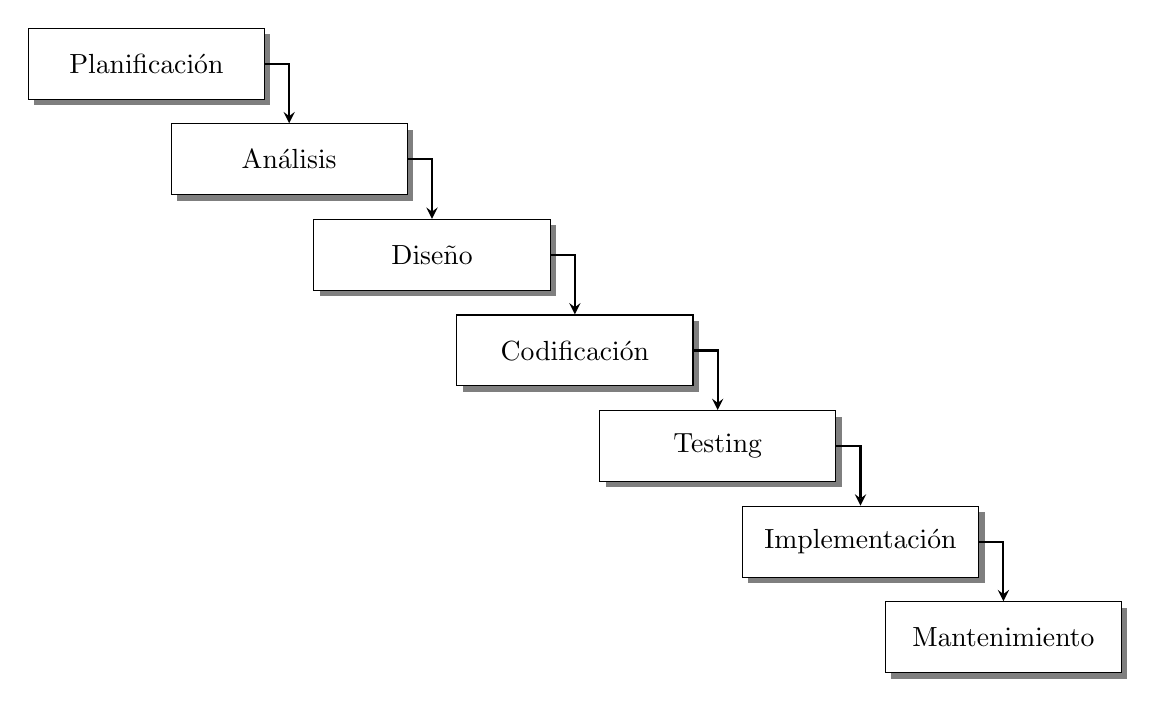
\begin{tikzpicture}[>=stealth,
   node distance = 3mm and -12mm,
     start chain = A going below right,
every node/.style = {draw, text width=28mm, minimum height=9mm, align=center,
                    inner sep=1mm, fill=white, drop shadow={fill=black},  on chain=A}
                  ]
\node {Planificación}; % A-1
\node {Análisis};
\node {Diseño};
\node {Codificación};
\node {Testing};
\node {Implementación};
\node {Mantenimiento};
%
\foreach \i [count=\j] in {2,...,7}
{
 \draw[->, thick] (A-\j) -| (A-\i);
}
\end{tikzpicture}
\caption{Esquema de un Modelo en cascada} \label{fig:M1}
\end{figure}

Sin embargo, como cualquier otra metodología software, es necesario tener en cuenta ciertas consideraciones imprescindibles para el transcurso del proyecto:

\begin{itemize}
   \item[$\bullet$] Como ya se había comentado, es necesario hacer hincapié en las etapas tempranas del modelo, ya que son
   las que van a definir de manera correcta los requisitos de la solución. De forma que, si no están bien establecidos, pueden 
   aparecer problemas en el resto de fases~\cite{wiegers2013software}.
   \item[$\bullet$] Esta metodología carece de iteraciones por lo que no es posible retroceder a las etapas anteriores.
   Hay que cerciorarse de que cada una de las fases se aprueban correctamente, de forma que sea seguro pasar a la
   fase siguiente.
   \item[$\bullet$] En la práctica, es recomendable marcar bien los tiempos de cada fase, marcando estimaciones de cada fase y contrastarlas con
   el tiempo real que ha supuesto realizarlas. Esta especie de monitorización se realizará periódicamente y se puede encontrar 
   en el \autoref{chap:A1}
\end{itemize}

\section{Estructura de la memoria} %%%%% Opcional

El resto de capítulos que conforman la memoria, son los que se resumen a continuación:

\begin{itemize}
   \item[$\bullet$] \textbf{Capítulo 2. Estudio estratégico}: corresponde al conocido apartado \textit{estado del arte}, en el que se realiza una labor 
   de estudio de aquellas soluciones relacionadas con \textit{nonogramas} dentro del mundo digital y que puedan ayudar a la identificación y extracción de requisitos.
   \item[$\bullet$] \textbf{Capítulo 3. Análisis del problema}: en este capítulo se expone la parte de especificación de requisitos,
    identificando aquellos que puedan repercutir negativamente al transcurso del proyecto.
   \item[$\bullet$] \textbf{Capítulo 4. Diseño de la solución}: se muestran las decisiones que se han tomado a nivel de arquitectura, patrones de diseño, 
   y tecnologías empleadas.
   \item[$\bullet$] \textbf{Capítulo 5. Desarrollo de la solución}: se comentan las distintas partes que han compuesto el aplicativo, cómo se comportan y 
   el funcionamiento interno de cada una de ellas, entrando en el apartado técnico.
   \item[$\bullet$] \textbf{Capítulo 6. Pruebas}: se muestran el conjunto de pruebas, que se han desarrollado para la posible identificación de 
   errores y posibles fallos en su ejecución, todas ellas divididas en tipos. 
   \item[$\bullet$] \textbf{Capítulo 7. Implementación y mantenimiento}: se explica el paso que se ha realizado para hacer que el aplicativo sea accesible
   para los usuarios y las medidas para su mantenimiento. 
   \item[$\bullet$] \textbf{Capítulo 8. Manual de uso}: presenta una pequeña demo con el fin de que el usuario se familiarice con el uso de
   la solución, mostrando capturas del mismo.
   \item[$\bullet$] \textbf{Capítulo 9. Conclusión y Trabajo Futuro}: contempla las conclusiones que se han obtenido durante la realización del trabajo y
   las mejoras que se tomarán para siguientes versiones del mismo.
   \item[$\bullet$] \textbf{Apéndices}: se muestran anexos relacionados con análisis de tiempos y apartados relacionados con la codificación del
   la solución y análisis de tiempos.
\end{itemize}

\chapter{Estudio estratégico}
\textit{Los \textit{nonogramas} junto otros gigantes rompecabezas de <<papel y lápiz>> tales como: sudoku, crucigramas, hundir la flota, ahorcado... se han adaptado a
una era en la que está gobernada por las nuevas plataformas tecnológicas. Y más concretamente, en estos tiempos de incertidumbre, confinamientos e incluso ocio han propiciado que estos
puzzles se hagan cada más presentes en nuestras vidas, alejándose una posible obsolescencia.}

\section{Nonogramas en la era Digital}

Pese a que la era Digital ofrece un amplio abanico de medios o plataformas que han incluido y popularizado estos rompecabezas, en
este apartado nos enfocaremos en el de las aplicaciones móviles.

Para que el estudio sea exhaustivo, se explorarán aquellas aplicaciones disponibles en las principales tiendas de aplicaciones para 
las plataformas \textit{Android} e \textit{iOS}, \textit{Google Play} y \textit{App Store} respectivamente.

\subsection{Nonograms Katana}
Nonograms Katana es una aplicación con una remarcada temática nipona, que permite al usuario resolver una gran variedad de \textit{nonogramas},
de una gran variedad de categorías y dimensiones, como se puede comprobar en la Figura~\ref{fig:katana2-1}.

\begin{figure}[H]
   \centering
   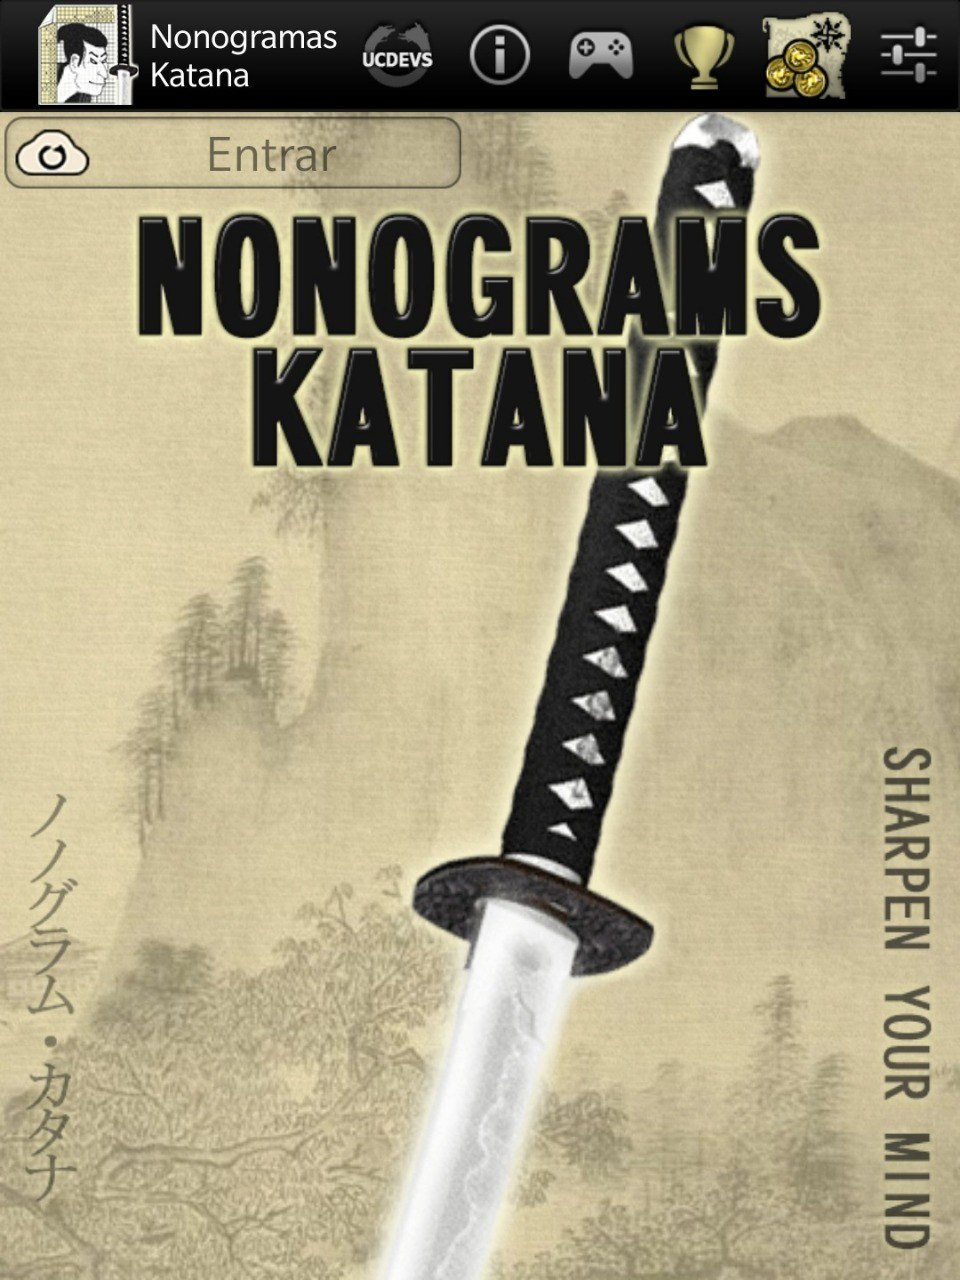
\includegraphics[scale=.15]{images/nonokatana1.jpg}
   \caption{Pantalla principala de Nonograms Katana}
   \label{fig:katana1}
 \end{figure}

 Además, como se puede apreciar en la Figura~\ref{fig:katana2-2}, se incluye la resolución de \textit{nonogramas} a color, en el que mediante un selector
 de colores el usuario pinta cada una de las celdas, resolviendo de este modo el \textit{nonograma}.

 \begin{figure}[H]
   \centering
   \begin{subfigure}[b]{0.47\linewidth}
     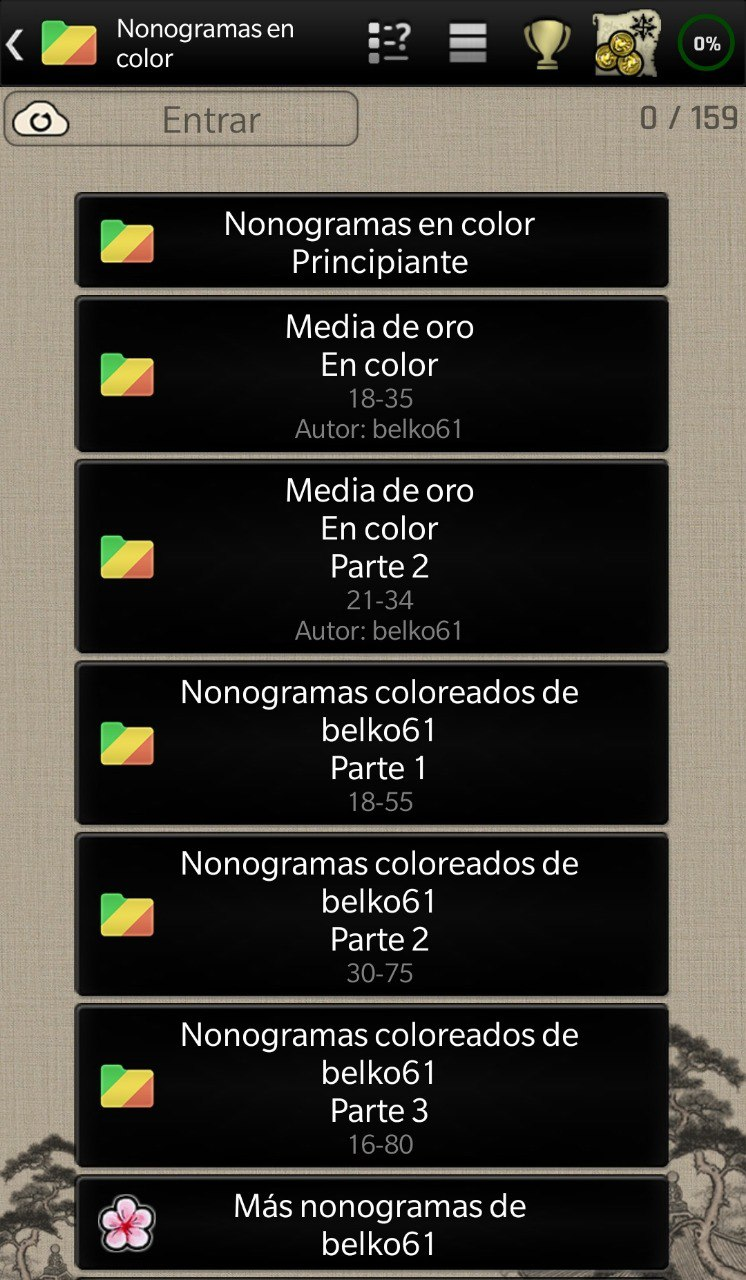
\includegraphics[width=\linewidth]{images/nonokatana2.jpg}
     \caption{Selector de niveles Nonogramas a color}
     \label{fig:katana2-1}
   \end{subfigure}
   \begin{subfigure}[b]{0.47\linewidth}
     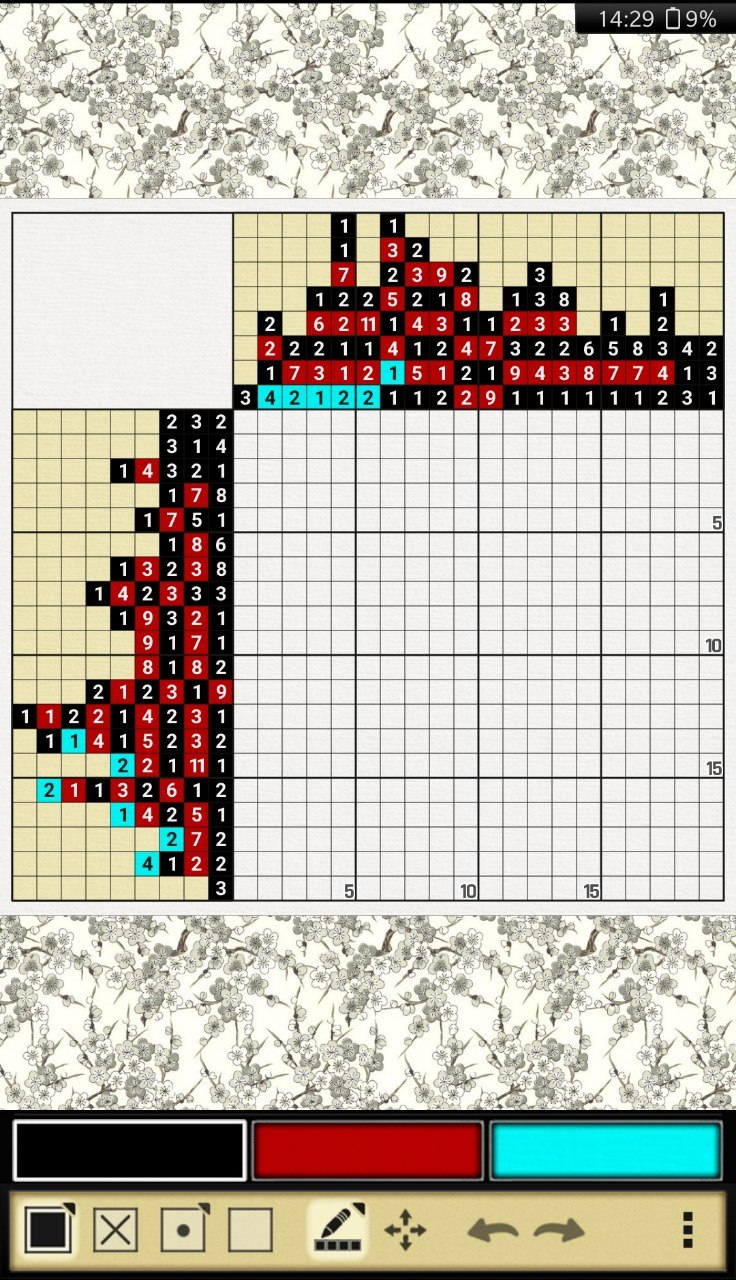
\includegraphics[width=\linewidth]{images/nonokatana3.jpg}
     \caption{Pantalla de resolución de un nivel 20x20 a color}
     \label{fig:katana2-2}
   \end{subfigure}
   \caption{Pantallas de Nonograms Katana con modalidad a color.}
   \label{fig:katana2}
 \end{figure}
 
 El aplicativo sigue la corriente clásica y no permite al usuario resolver los \textit{nonogramas} bajo un número determinado de \textit{vidas} 
 o intentos \textit{(disminuyendo su valor al pulsar sobre celdas erróneas)}, siendo algo tediosa la experiencia de juego, ya que puede acarrear fallos
 durante su resolución.

 Una característica notable de la aplicación es la de permitir al usuario crear sus propios \textit{nonogramas}, compartirlos con la comunidad, y resolver los de
 otros usuarios. Sin embargo, está propiedad no es su principal función y aparece bloqueda si no estás registrado, además de estar limitada por restricciones como los de la 
 Figura~\ref{fig:katana3}.

 El aplicativo presenta la propiedad de multilenguaje, no obstante, este presenta errores en sus traducciones, como se puede comprobar en la figura anteriormente
 citada.

 \begin{figure}[H]
   \centering
   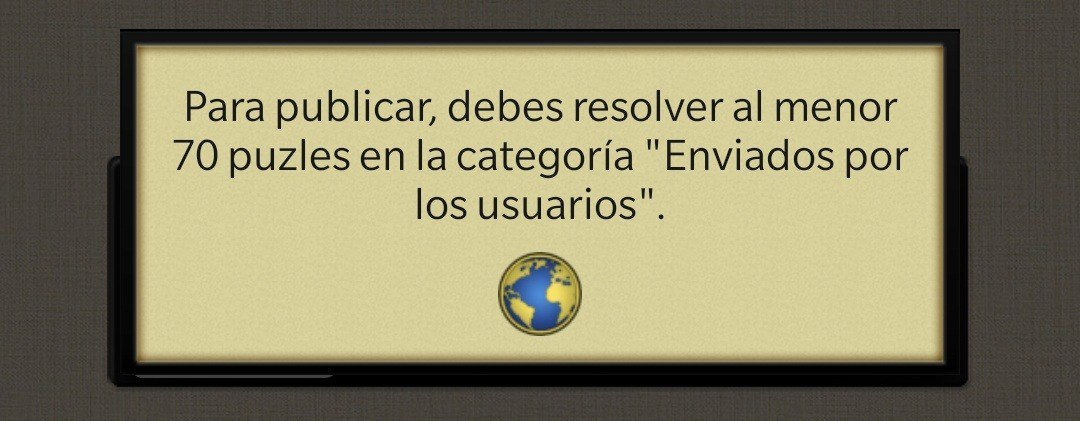
\includegraphics[scale=.175]{images/nonokatana4.jpg}
   \caption{Modal de restricción en publicación en Nonograms Katana}
   \label{fig:katana3}
 \end{figure}
 

\subsection{Nonogram.com - Picture cross number puzzle}

Una de las aplicaciones más descargadas dentro de la categoría puzzle con más de diez millones de descargas en la tienda \textit{Google Play}, 
presenta una interfaz amigable y limpia.

Hace un buen uso de animaciones, destacando la experiencia de juego, algunas bastante remarcables como cuando la que se muestra en la 
Figura~\ref{fig:picture1-2}, en cuanto finalizas un nivel.

\begin{figure}[h!]
   \centering
   \begin{subfigure}[b]{0.45\linewidth}
     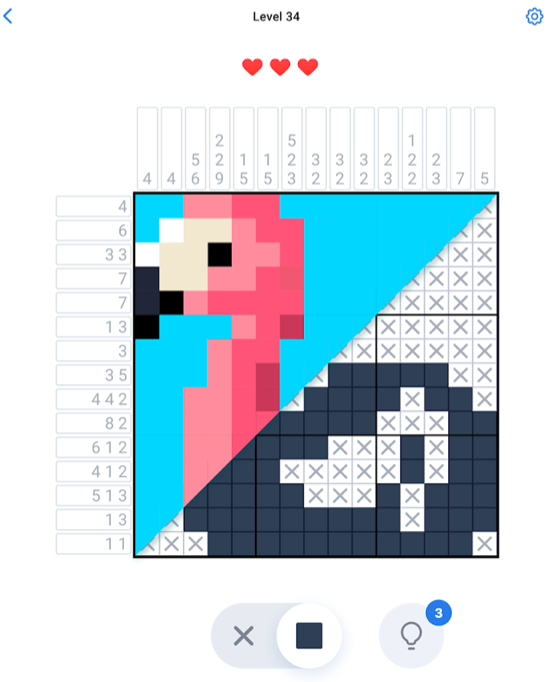
\includegraphics[width=\linewidth]{images/picturecross1.png}
     \caption{Pantalla de resolución de un nivel 15x15}
     \label{fig:picture1-1}
   \end{subfigure}
   \begin{subfigure}[b]{0.45\linewidth}
     
\includegraphics[width=\linewidth]{images/picturecross2.png}
     \caption{Pantalla de felicitación al resolver el nivel}
     \label{fig:picture1-2}
   \end{subfigure}
   \caption{Pantallas de Nonogram.com}
   \label{fig:picture1}
 \end{figure}

Como característica extra de juego, como se visualiza en la Figura~\ref{fig:picture1-1}, la barra inferior de juego incorpora un botón llamado \textit{Pista}, 
con el que después de ser seleccionado, 
el usuario puede clicar sobre una celda determinada y descubrir si es correcta sin restar una vida, teniendo limitada esta opción a tres usos por nivel.

\begin{figure}[H]
   \centering
   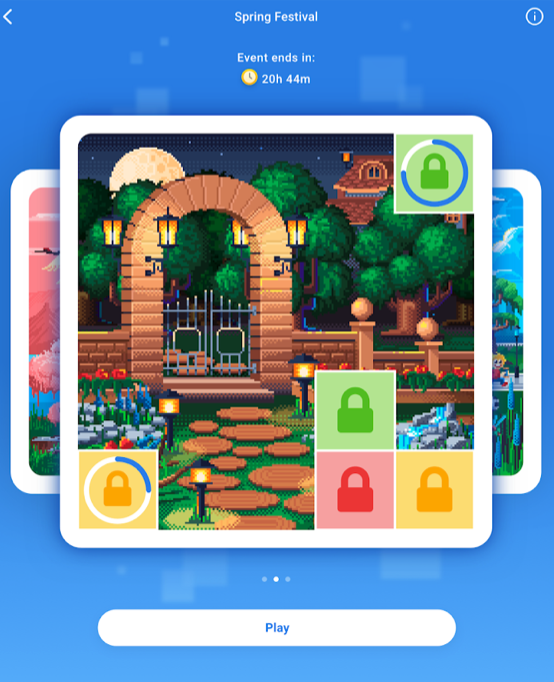
\includegraphics[scale=.25]{images/picturecross3.png}
   \caption{Pantalla de Evento Primavera de Nonogram.com}
   \label{fig:picture2}
 \end{figure}

En el aplicativo, de forma recurrente, aparecen \textit{Eventos} en los que el usuario puede resolver un conjunto de \textit{nonogramas} especiales relacionados
con una temática concreta, representada en la Figura~\ref{fig:picture2}.
 
La solución, como se ha podido comprobar, es de las más completas de las disponibles, no obstante, incluye publicidad excesivamente intrusiva para el usuario,
presente en casi todas sus funcionalidades, que entorpecen la experiencia de juego, incluso llegando a entorpecer al jugador.

\subsection{Nono Infinite}
Este producto destaca por su interfaz \textit{arcade}, con una clara intención de ser dirigida para todos los públicos, constrantando colores muy vivos,
con formas que recuerdan mucho a juegos clásicos para niños, se puede ver reflejado en las Figuras~\ref{fig:infinite1}.

\begin{figure}[h!]
   \centering
   \begin{subfigure}[b]{0.49\linewidth}
     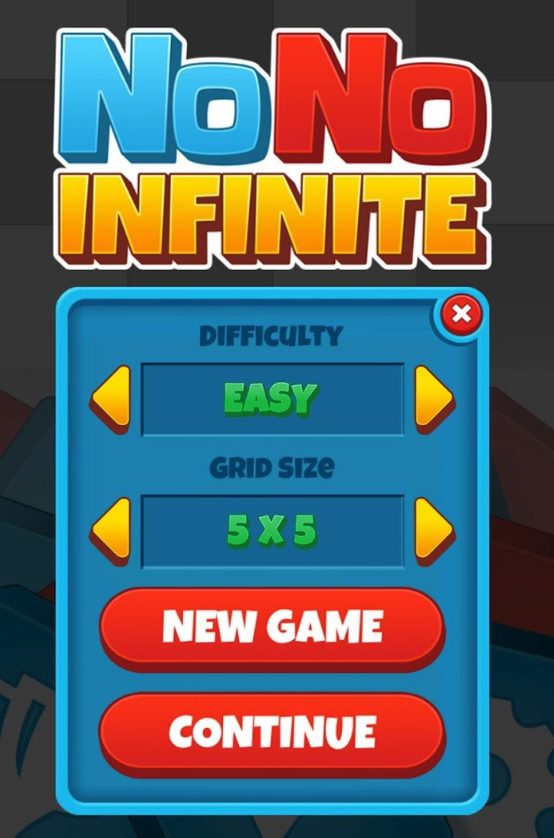
\includegraphics[width=\linewidth]{images/infinite1.png}
     \caption{Pantalla selector de nivel}
     \label{fig:infinite1-1}
   \end{subfigure}
   \begin{subfigure}[b]{0.49\linewidth}
     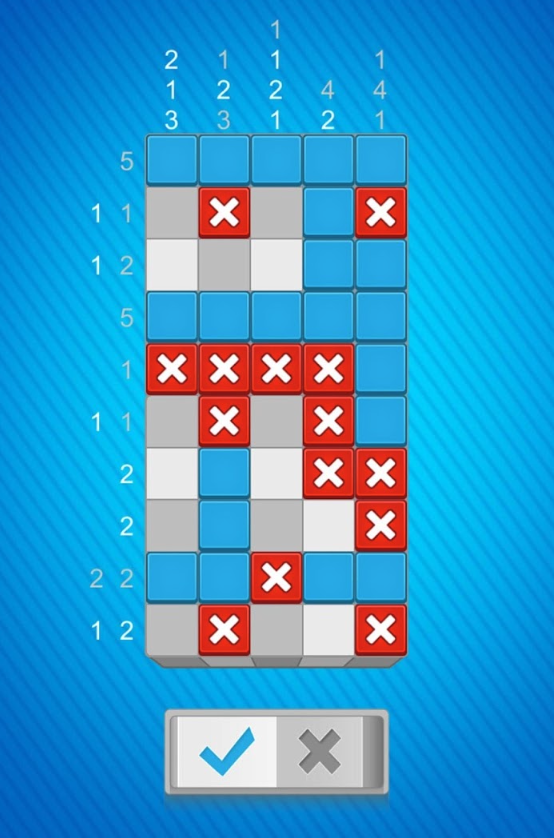
\includegraphics[width=\linewidth]{images/infinite2.png}
     \caption{Pantalla de resolución de un nivel 5x10}
     \label{fig:infinite1-2}
   \end{subfigure}
   \caption{Pantallas de selección de nivel y juego de Nono Infinite}
   \label{fig:infinite1}
 \end{figure}

Como peculiaridad, presenta \textit{nonogramas} de dimensiones poco usuales que difieren mucho de los clásicos, como el 5x10 presente en la
Figura~\ref{fig:infinite1-2}. Así mismo, permite cambiar la dificultad de los niveles manteniendo las dimensiones del mismo, sin embargo,
esta puede parecer un poco "\textit{artificial"} ya que únicamente aumenta las distancias de las celdas correctas.

Resulta interesante cómo la solución aprovecha el apartado del tutorial, para habituar al usuario de forma interactiva con las reglas clásicas de los 
\textit{nonogramas}, controles del mismo y consejos más avanzados, sobretodo para niveles más complejos, Figura~\ref{fig:infinite2}.

\begin{figure}[H]
   \centering
   \begin{subfigure}[b]{0.4\linewidth}
     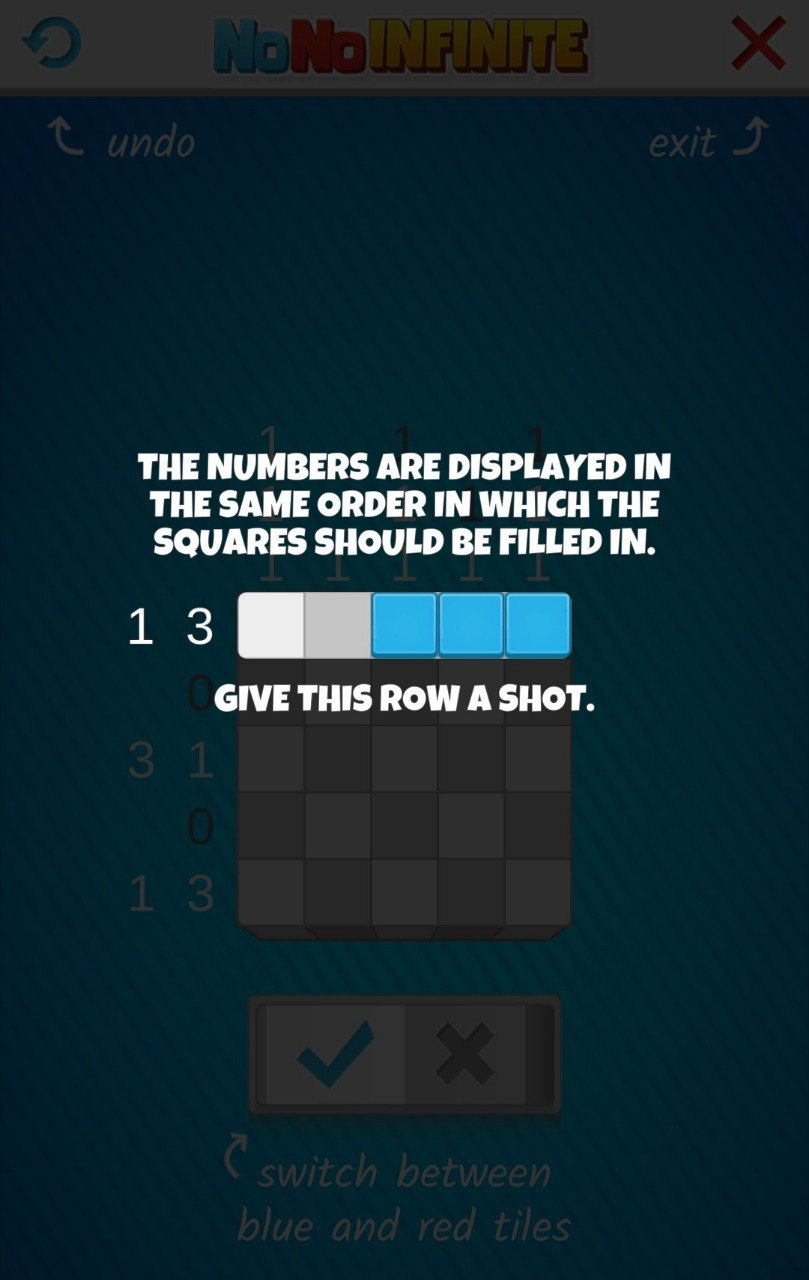
\includegraphics[width=\linewidth]{images/infinite3.jpg}
   \end{subfigure}
   \begin{subfigure}[b]{0.4\linewidth}
     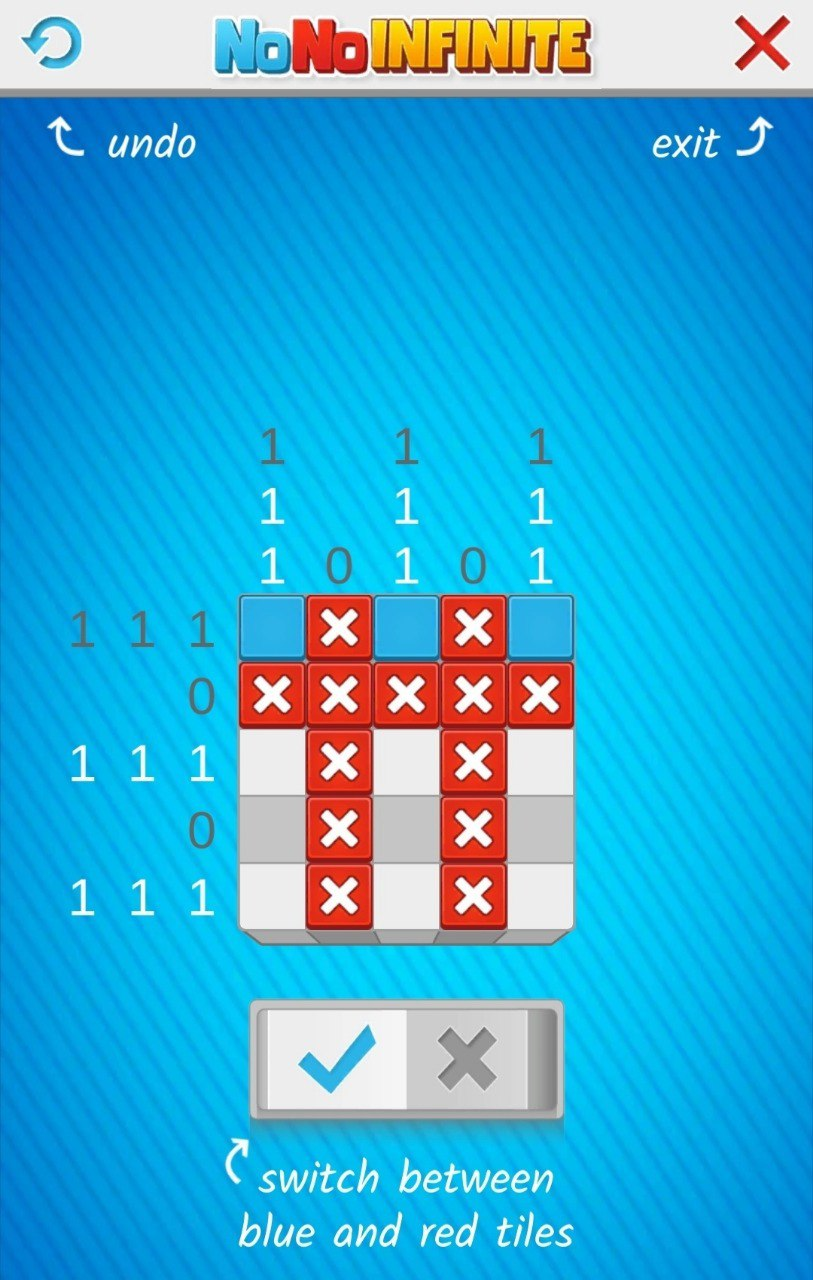
\includegraphics[width=\linewidth]{images/infinite4.jpg}
   \end{subfigure}
   \caption{Pantallas de tutorial en Nono Infinite}
   \label{fig:infinite2}
 \end{figure}

 \subsection{Family Crest Nonogram}

 Family Crest Nonogram es un juego que, pese a que no destaque por su apartado gráfico e interfaz de usuario, presenta muchas características que lo diferencian
 del resto de soluciones del género.

 Lo más remarcable de la aplicación es que tenga establecido su uso en modo \textit{landscape} (apaisado), adaptándose al formato de la mayoría de géneros
 de juegos de móvil. Sin embargo, este puede ser un punto negativo para muchos, ya que priva al jugador la esencia de estar jugando a un pasatiempo,
 recordándo más a la de un \textit{videojuego}.

 \begin{figure}[h!]
  \centering
  \begin{subfigure}[b]{0.49\linewidth}
    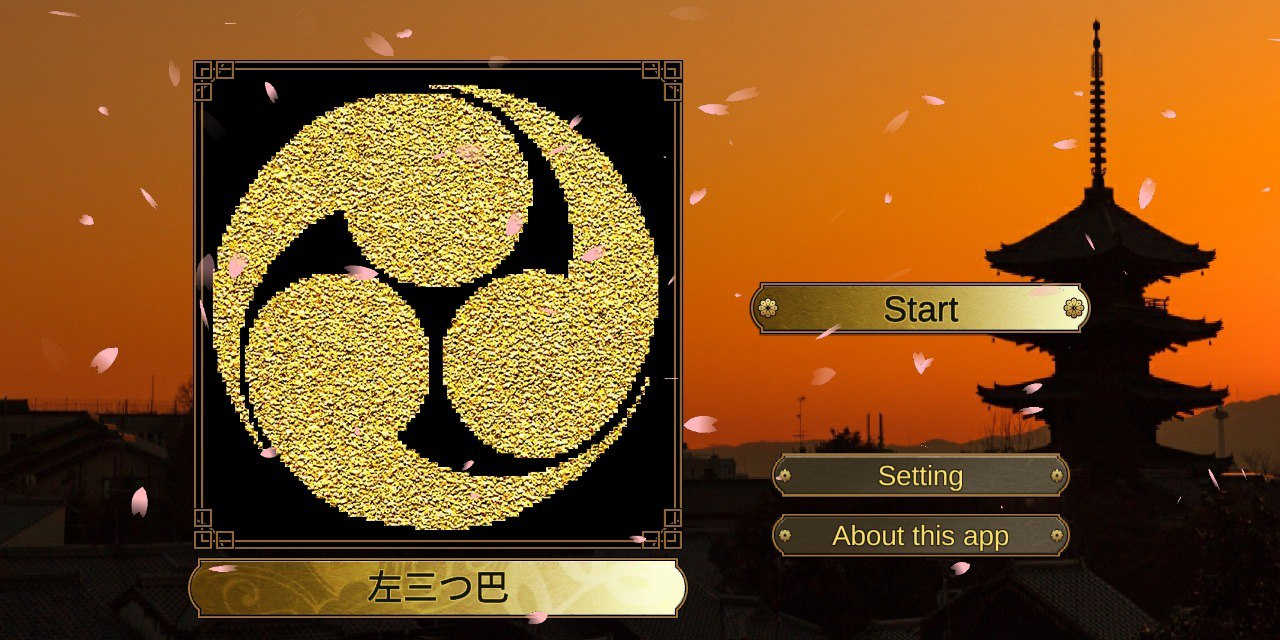
\includegraphics[width=\linewidth]{images/familycrest1.jpg}
    \caption{Pantalla principal}
    \label{fig:family1-1}
  \end{subfigure}
  \begin{subfigure}[b]{0.49\linewidth}
    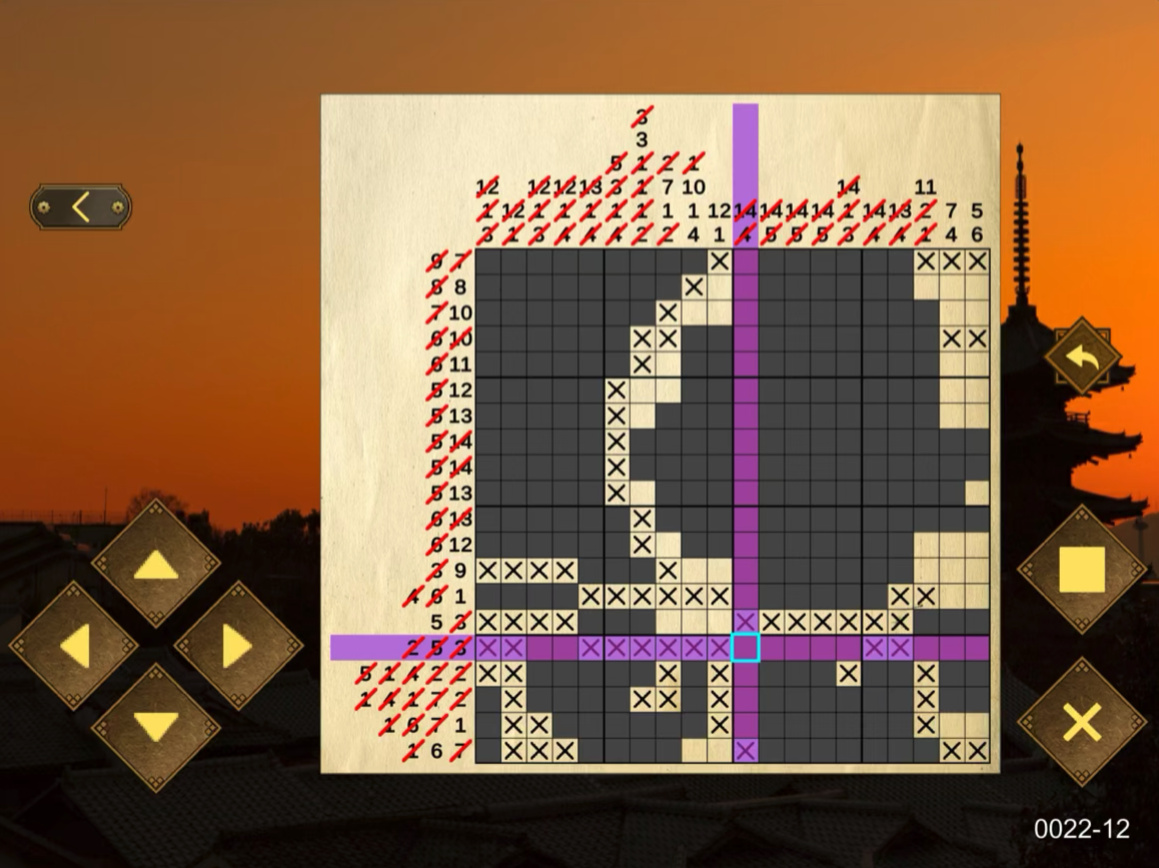
\includegraphics[width=\linewidth]{images/familycrest2.png}
    \caption{Pantalla de resolución de un nivel 20x20}
    \label{fig:family1-2}
  \end{subfigure}
  \caption{Pantallas de Family Crest}
  \label{fig:family1}
\end{figure}

No obstante, su experiencia de juego es muy notable, ya que presenta una \textit{cruceta} (para moverse por cada una de las celdas) 
y botones físicos de acción que facilitan un mayor control,
Figura~\ref{fig:family1-2}, además de incorporar una música ambiente que acompaña al usuario cada vez que  está jugando un nivel.

\section{Ánalisis de las aplicaciones}

Al analizar las aplicaciones enfocadas al submundo de los \textit{nonogramas}, vemos que siguen un patrón de similitudes, que resultan sustanciales 
para el desarrollo de una solución del género rompecabezas, además de ciertas peculiaridades que parecen interesantes para su inclusión en la solución.
Es importante también remarcar y apartar aquellas características que puedan ser perjudiciales para una primera versión de la solución.
A continuación, se muestra un tabla representativa de cada una de las características estudiadas, donde se objetarán su final inclusión en el aplicativo:

\renewcommand\theadalign{b}
\renewcommand\theadfont{\bfseries}
\renewcommand\theadgape{\Gape[1pt]}
\renewcommand\cellgape{\Gape[1pt]}
\newcommand{\cmark}{{\ding{51}}}
\newcommand{\xmark}{{\ding{55}}}
\begin{table}[H]
  \caption{Comparativa de características entre aplicaciones de interés y su inclusión como requisito}
    \begin{tabular}{ | c | c | c | c | c | c |}
      \hline
      \thead{Característica \\ encontrada} & \thead{Nonogram \\ Katana} & \thead{Nonograma.com \\ Picture cross} & \thead{Nono \\ Infinite} & \thead{Family \\ Crest} & \thead{Incluido como \\ requisito} \\
      \hline
      \makecell{Aplicación \\ multiplataforma} &  \cmark  & \cmark  & \xmark & \cmark & \cmark \\
      \hline
      \makecell{Temática \\ especial} &  \cmark  & \xmark  & \cmark & \cmark & \cmark \\
      \hline
      \makecell{Creación \\ nonogramas} &  \cmark*  & \xmark  & \xmark & \xmark & \cmark \\
      \hline
      \makecell{Opción de \\ autoguardado} &  \cmark  & \cmark  & \xmark & \xmark & \cmark* \\
      \hline
      \makecell{Registro de \\ usuario} &  \cmark  & \xmark  & \xmark & \xmark & \xmark \\
      \hline
      \makecell{Sincronización \\de niveles en nube} &  \cmark  & \xmark  & \xmark & \xmark & \cmark \\
      \hline
      \makecell{Juego \\ con \textit{vidas}} &  \xmark  & \cmark  & \xmark & \xmark & \cmark* \\
      \hline
      \makecell{Música \\ ambiente} &  \xmark  & \xmark  & \xmark & \cmark & \xmark \\
      \hline
      \makecell{Botón de \\ pistas} &  \xmark  & \cmark  & \xmark & \xmark & \xmark \\
      \hline
      \makecell{Botones físicos \\ de acción} &  \cmark  & \cmark  & \cmark & \cmark & \xmark \\
      \hline
      \makecell{Variedad de\\ visuales} &  \cmark  & \xmark  & \xmark & \xmark & \cmark \\
      \hline
      \makecell{Multi- \\ idioma} &  \cmark*  & \cmark  & \xmark & \xmark & \cmark \\
      \hline
      \makecell{Eventos \\ especiales} &  \xmark  & \cmark  & \xmark & \xmark & \xmark \\
      \hline
      \makecell{Nonogramas \\ a color} &  \cmark  & \xmark  & \xmark & \xmark & \xmark \\
      \hline
      \makecell{Tutorial \\ de juego} &  \cmark  & \cmark  & \cmark & \xmark & \cmark \\
      \hline
      \makecell{Sección \\ Leaderboard} &  \cmark  & \cmark  & \xmark & \xmark & \xmark \\
      \hline
      \makecell{Selector de \\ niveles} &  \cmark  & \xmark  & \xmark & \cmark & \cmark \\
      \hline
    \end{tabular}
    \label{fig:table1}
\end{table}

La inclusión de las características de la Tabla~\ref{fig:table1} se ven indicadas mediante la siguiente simbología:

\begin{enumerate}
	\item \cmark : Característica incluida en el aplicativo.
	\item \xmark : Característica no incluida en el aplicativo.
	\item \cmark* : Característica incluida en el aplicativo con ciertos matices.
\end{enumerate}

\section{Propuesta}
Visualizando las características reflejadas en la Tabla~\ref{fig:table1} sacamos la siguientes conclusiones de cara a la creación de la primera
versión de la aplicación como producto:

\begin{itemize}
  \item[$\bullet$] Ya que la mayoría de apps estudiadas son multiplataforma, el aplicativo funcionará para ambas plataformas \textit{Android} e \textit{iOS}.
  \item[$\bullet$] Seguirá una temática especial con el fin de diferenciarlas del resto, además de ir alternando entre temas diversos cambiando
  la interfaz de usuario.
  \item[$\bullet$] Tanto la resolución como la creación de los nonogramas será una de las funciones de la solución, sin ningún tipo de restricción.
  \item[$\bullet$] El usuario podrá usar \textit{servicios in-cloud} como: sincronización en nube o acceso a la base de datos sin tener que registrarse.
  \item[$\bullet$] La aplicación tendrá posibilidad multi-idioma, teniendo disponible inglés y español para esta primera versión, sin ningún tipo de errata.
  \item[$\bullet$] Se podrán jugar niveles de \textit{nonogramas} de diferentes dimensiones clásicas, recordando a los de los medios físicos tradicionales,
  previamente explicado su uso por un tutorial intuitivo. 
  \item[$\bullet$] Durante la resolución del nonograma, el usuario podrá resolverlo con una interfaz minimalista, en ausencia de botones físicos,
  además de poder alternar entre resolución con y sin \textit{vidas}.
  \item[$\bullet$] Muchas de las características estudiadas se han tomado como no esenciales y quedarán descartadas para la primera versión.
\end{itemize}

\chapter{Análisis del problema}
\textit{La Ingeniería de Requisitos (IR) es el área más importante de la Ingeniería de Software y posiblemente de todo el 
ciclo de vida de una solución software (SDLC)~\cite{chakraboty2012requirements}. Esta etapa es la responsable de que los 
requisitos recién detectados, aún incompletos e imprecisos, se transformen en especificaciones formales del aplicativo final.}

\section{Especificación de requisitos}
Para llevar a cabo la especificación total de requisitos se seguirá la norma tradicional establecida por el estándar internacional 
IEEE Std 830-1998~\cite{8559686}, elegido por una gran mayoría de jefes de departamentos software por su gran agilidad en la fase de gestión 
de requisitos~\cite{guzman2018impacto}.

A continuación, de acuerdo a la normativa ISO elegida, se mostrarán los contenidos acompañados por diagramas y buenas prácticas.

\subsection{Propósito}
El propósito de esta sección es la de definir y formalizar los requerimientos que debe incorporar el \textit{MVP} del aplicativo, facilitando
y guiando el desarrollo del mismo.

\subsection{Ámbito}
El ámbito, como se ha comentado en capítulos anteriores, es el de las aplicaciones móviles disponibles en plataformas \textit{iOS} y 
\textit{Android}.

El aplicativo en su versión \textit{MVP} adoptará el nombre provisional de \textit{NonoChallenge}, compuesto por el juego de palabras:
 \textit{Nonograma} junto con el término anglosajón \textit{Challenge} (reto).
En el cual, el usuario hará uso de sus servicios propios y \textit{en nube} tales como inicios de sesión, interacción con base de datos y
sincronización.

\subsection{Terminología}
Los términos relacionados con la ontología del sistema se ven enumerados y descritos por la Tabla~\ref{fig:table2}.

\begin{table}[H]
  \caption{Glosario de términos ontológicos del aplicativo}
    \begin{tabular}{ | c | c |}
      \hline
      \thead{Término} & \thead{Descripción} \\
      \hline
      \makecell{Usuario} &  Persona que hará el uso del conjunto de funcionalidades del aplicativo final  \\
      \hline
      \makecell{Nonograma} &  \makecell{Rompecabezas de MxN dimensiones}  \\
      \hline
      \makecell{Nivel} &  Nonograma a crear o resolver por el Usuario\\
      \hline
      \makecell{Progreso} &  \makecell{Datos relacionados con la persistencia de la resolución de un nivel} \\
      \hline
    \end{tabular}
    \label{fig:table2}
\end{table}

Por otra parte, los términos técnicos que componen el sistema son los que siguen:

\begin{table}[H]
    \caption{Glosario de términos técnicos del aplicativo}
      \begin{tabular}{ | c | c |}
        \hline
        \thead{Término} & \thead{Descripción} \\
        \hline
        \makecell{Nombre \\ de usuario} &  \makecell{Nombre que adoptará el Usuario de forma opcional para su\\identificación en el aplicativo.}  \\
        \hline
        \makecell{Email} &  \makecell{Cuenta de correo que hará uso el usuario para acceder a los servicios \textit{en nube}}  \\
        \hline
        \makecell{Fecha de \\ publicación} &  Fecha en la que el usuario crea y publica un nivel  \\
        \hline
        \makecell{Figura} &  Nombre identificativo de un nonograma \\
        \hline
        \makecell{Vidas} &  Número de intentos en la resolución de un nivel \\
        \hline
        
      \end{tabular}
      \label{fig:table3}
  \end{table}

  \subsection{Modelo de Dominio}
  Una vez introducida la términología propia del sistema, para un mayor entendimiento del contexto del mismo, se representa un  
  diagrama de clases de acuerdo a las reglas clásicas UML, como se pude visualizar en la Figura~\ref{fig:dom1}.

  \begin{figure}[H]
    \centering
  \begin{tikzpicture}
    \begin{umlpackage}[fill=black!10]{Sistema}
      \umlclass[x=1,y=1]{Usuario}{uid : string \\ nombreUsuario : string? \\ email : string? \\ numCompletados : int}{}
      \umlclass[x=2,y=-3.8]{Nivel}{uid : string \\ fechaPub : datetime? \\ figura : string \\ vidas : int}{}
      \umlclass[x=9,y=-3.8]{Nonograma}{  width : int \\ height : int \\ celdasCorrectas : List<int>}{}
      \umlclass[x=8,y=1]{<<data>> Progreso}{id : int \\ completado : int \\ celdasMarcadas : string? \\ celdasDescartadas : string? \\ vidas : int}{}
    \end{umlpackage}
      
    \umlassoc[pos=0.6,arg=crea,mult1=1,mult2=0*, anchors=-130 and 130] {Usuario}{Nivel}
    \umlassoc[pos=0.6,arg=resuelve,mult1=1,mult2=0*, anchors=-60 and 55] {Usuario}{Nivel}
    \umlassoc[pos=0.7,arg=contiene,mult1=1,mult2=1] {Nivel}{Nonograma}
    \umlassoc[arg=tiene,mult1=1,mult2=0..1] {Nivel}{<<data>> Progreso}
    % \umlassoc[geometry=-|-, arg1=tata, mult1=*, pos1=0.3, arg2=toto, mult2=1, pos2=2.9, align2=left]{C}{B}
    % \umlunicompo[geometry=-|, arg=titi, mult=*, pos=1.7, stereo=vector]{D}{C}
    % \umlaggreg[arg=tutu, mult=1, pos=0.8, angle1=30, angle2=60, loopsize=2cm]{D}{D}
    % \umlinherit[geometry=-|]{D}{B}
    \end{tikzpicture}
    \caption{Diagrama del modelo de dominio}
   \label{fig:dom1}
  \end{figure}

  A continuación, se comenta la función de cada de una de las clases conceptuales y se enumeran en las Tablas~\ref{fig:table3}-~\ref{fig:table6} 
  los atributos que las componen. \textit{(La anotación ? al lado del tipo refleja su posibilidad de
  nulidad en el sistema.)}
  

  \textbf{$\bullet$ Clase Usuario}: Conjunto de datos del usuario relacionados con el sistema.

  \begin{table}[H]
    \centering
    \caption{Atributos de la clase Usuario}
      \begin{tabular}{ | c | c |}
        \hline
        \thead{Atributos de Usuario} & \thead{Descripción} \\
        \hline
        \makecell{uid\\\textit{\textit{string}}} & \makecell{Cadena de caracteres único que identifica al usuario a \\nivel interno}\\
        \hline
        \makecell{nombre de Usuario\\\textit{string?}} & Pseudónimo único a elegir por el usuario en el sistema \\
        \hline
        \makecell{email\\\textit{string?}} &  Cuenta de correo de registro única para el usuario\\
        \hline
        \makecell{numCompletados\\\textit{int}} &  \makecell{Número de niveles completados por el usuario} \\
        \hline
      \end{tabular}
      \label{fig:table3}
  \end{table}

  \textbf{$\bullet$ Clase Nivel}: Muestra las características de un determinado nivel a resolver.

  \begin{table}[H]
    \centering
    \caption{Atributos de la clase Nivel}
      \begin{tabular}{ | c | c |}
        \hline
        \thead{Atributos de Nivel} & \thead{Descripción} \\
        \hline
        \makecell{uid\\\textit{\textit{string}}} & \makecell{Cadena de caracteres único que identifica al nivel}\\
        \hline
        \makecell{fecha de Publicación\\\textit{dateTime?}} & Fecha de creación del nonograma en caso de llegar a publicarse \\
        \hline
        \makecell{figura\\\textit{string}} &  Nombre del nivel mostrado una vez resuelto\\
        \hline
        \makecell{vidas\\\textit{int}} &  \makecell{Número de intentos que dispone un usuario para la resolución de \\un nivel} \\
        \hline
      \end{tabular}
      \label{fig:table4}
  \end{table}

  \textbf{$\bullet$ Clase Progreso}: Clase de persistencia que contiene los datos durante la resolución de un nivel.

  \begin{table}[H]
    \centering
    \caption{Atributos de la clase Progreso}
      \begin{tabular}{ | c | c |}
        \hline
        \thead{Atributos de Progreso} & \thead{Descripción} \\
        \hline
        \makecell{id\\\textit{int}} & \makecell{Número de identificación del progreso de un determinado nivel}\\
        \hline
        \makecell{completado\\\textit{int}} & \makecell{Indica con un 1 si el nivel está resuelto y 0 si no lo está\\
        (simulando un dato de tipo booleano)}\\
        \hline
        \makecell{celdasMarcadas\\\textit{string}} &  \makecell{Números de las celdas pintadas separados por delimitadores\\
        (simulando un dato de tipo lista de enteros)}\\
        \hline
        \makecell{celdasDescartadas\\\textit{string}} &  \makecell{Números de las celdas descartadas separados por delimitadores\\
        (simulando un dato de tipo lista de enteros)}\\
        \hline
        \makecell{vidas\\\textit{int}} &  \makecell{Números de vidas que dispone el usuario en ese momento}\\
        \hline
      \end{tabular}
      \label{fig:table5}
  \end{table}
  \hfill 

  \textbf{$\bullet$ Clase Nonograma}: Contiene los datos del nonograma de un determinado nivel.

  \begin{table}[H]
    \centering
    \caption{Atributos de la clase Nonograma}
      \begin{tabular}{ | c | c |}
        \hline
        \thead{Atributos de Nonograma} & \thead{Descripción} \\
        \hline
        \makecell{width\\\textit{int}} & \makecell{Número de filas de celdas que compone el Nonograma}\\
        \hline
        \makecell{height\\\textit{int}} & Número de columnas de celdas que compone el Nonograma \\
        \hline
        \makecell{celdasCorrectas\\\textit{List<int>}} & \makecell{Lista de los números de celdas que componen \\
        la solución del Nonograma} \\
        \hline
      \end{tabular}
      \label{fig:table6}
  \end{table}

  \subsection{Límites del Sistema}
  Para representar los límites de la aplicación, se emplea un diagrama de contexto en el que se muestra la jerarquía de los actores 
  que van a interactúan con el aplicativo.

\tikzumlset{fill usecase=white}
\begin{figure}[H]
  \centering
\begin{tikzpicture}
    \begin{umlsystem}[x=5,y=-3,fill=black!10] {Aplicativo} % empty title
        % \umlusecase[name=a,width=1.5cm] {Use case}
        % \umlusecase[name=b,x=6,width=2.5cm] {Use case b}
        % \umlusecase[name=c,x=6,y=-3,width=2.5cm] {Use case c}
        % \umlusecase[name=d,y=-3,width=2.5cm] {Use case d}
    \end{umlsystem}


    \umlactor[y=-1] {Usuario}
    \umlactor[y=-4] {Usuario Registrado}

    \umlassoc{Usuario}{Aplicativo}
    \umlinherit{Usuario Registrado}{Usuario}
    
    % \umlextend{a}{b}
    % \umlinclude{c}{d}

    % manual versions of the above
    % \draw [tikzuml dependency style] (a) -- node[above] {$\ll \text{extend} \gg$} (b);
    % \draw [tikzuml dependency style] (d) -- node[above] {$\ll \text{include} \gg$} (c);

    % bent association
  \end{tikzpicture}
  \caption{Diagrama de Contexto del aplicativo}
   \label{fig:dom2}
\end{figure}

Como se puede apreciar en el diagrama de la Figura~\ref{fig:dom2}, únicamente van a interacutar dos actores con el sistema: i) el usuario sin registro,
que emplea únicamente las funciones locales del sistema y ii) el usuario registrado, que podrá emplear tanto las funciones locales como
\textit{en nube} del aplicativo.

\subsection{Restricciones del Sistema}

En este apartado se muestran algunas de las restricciones que pueden impedir algunas de las funcionalidades que ofrece el sistema
al usuario, vistos en la Tabla ~\ref{fig:table7}.

\begin{table}[H]
  \centering
  \caption{Restricciones del sistema}
    \begin{tabular}{ | c | c |}
      \hline
      \thead{Restricción} & \thead{Descripción} \\
      \hline
      \makecell{Memoria del\\ dispositivo} & \makecell{Posibilidad de que el dispositivo no tenga suficiente memoria
      \\disponible para guardar el progreso de la resolución de los niveles.\\\textit{Probabilidad prácticamente despreciable} }\\
      \hline
      \makecell{Conexión a\\internet} & \makecell{Las funcionalidades \textit{en nube} requieren de conexión a internet\\ para poder 
      llegar a usarse.} \\
      \hline
      \makecell{Cuenta\\de Google} &  \makecell{El usuario pueder carecer de una cuenta de correo de Google\\necesaria para hacer uso de las funcionalidades 
      \textit{en nube}.} \\
      \hline
    \end{tabular}
    \label{fig:table7}
\end{table}

\subsection{Características del Sistema}
Una vez vistas las limitaciones y restricciones del sistema, se pueden analizar las características finales a incorporar en la aplicación.





\chapter{Diseño de la solución}
\textit{El desarrollo de una aplicación multiplataforma es una opción cada vez más a tener en 
cuenta dentro del ámbito del desarrollo móvil~\cite{10.1145/3241739}. La mayor parte de desarrollos
se van a querer destinar a las principales plataformas móviles, 
con el fin de llegar al máximo número de usuarios posibles.
}

\section{Tecnología empleada}
Como se había decidido en el segundo capítulo, la realización de este \textit{MVP} irá dirigido para las
plataformas móviles: \textit{Android} e \textit{iOS}. El desarrollo de una aplicación \textit{nativa} para 
cada sistema, evidentemente, no sería factible, ya que implicaría el doble de esfuerzo en la codificación,
testing y mantenimiento del producto~\cite{10.1145/2480362.2480464}.

Por ello, es necesario el uso de un \textit{framework} de ámbito multiplataforma que nos proporcione un
soporte para ambas plataformas. En este caso, se ha optado por la prometedora herramienta de desarrollo
impulsada por \textit{Google}: \textit{Flutter}.

\subsection{Flutter y Dart}
\textit{Flutter} junto a su lenguaje de programación principal, \textit{Dart}, buscan 
aproximar al usuario la apariencia y rendimiento 
propio al de un desarrollo \textit{nativo}, aprovechando todas las ventajas que proporciona 
un \textit{framework multiplataforma}~\cite{7934674}.

\begin{figure}[H]
    \centering
    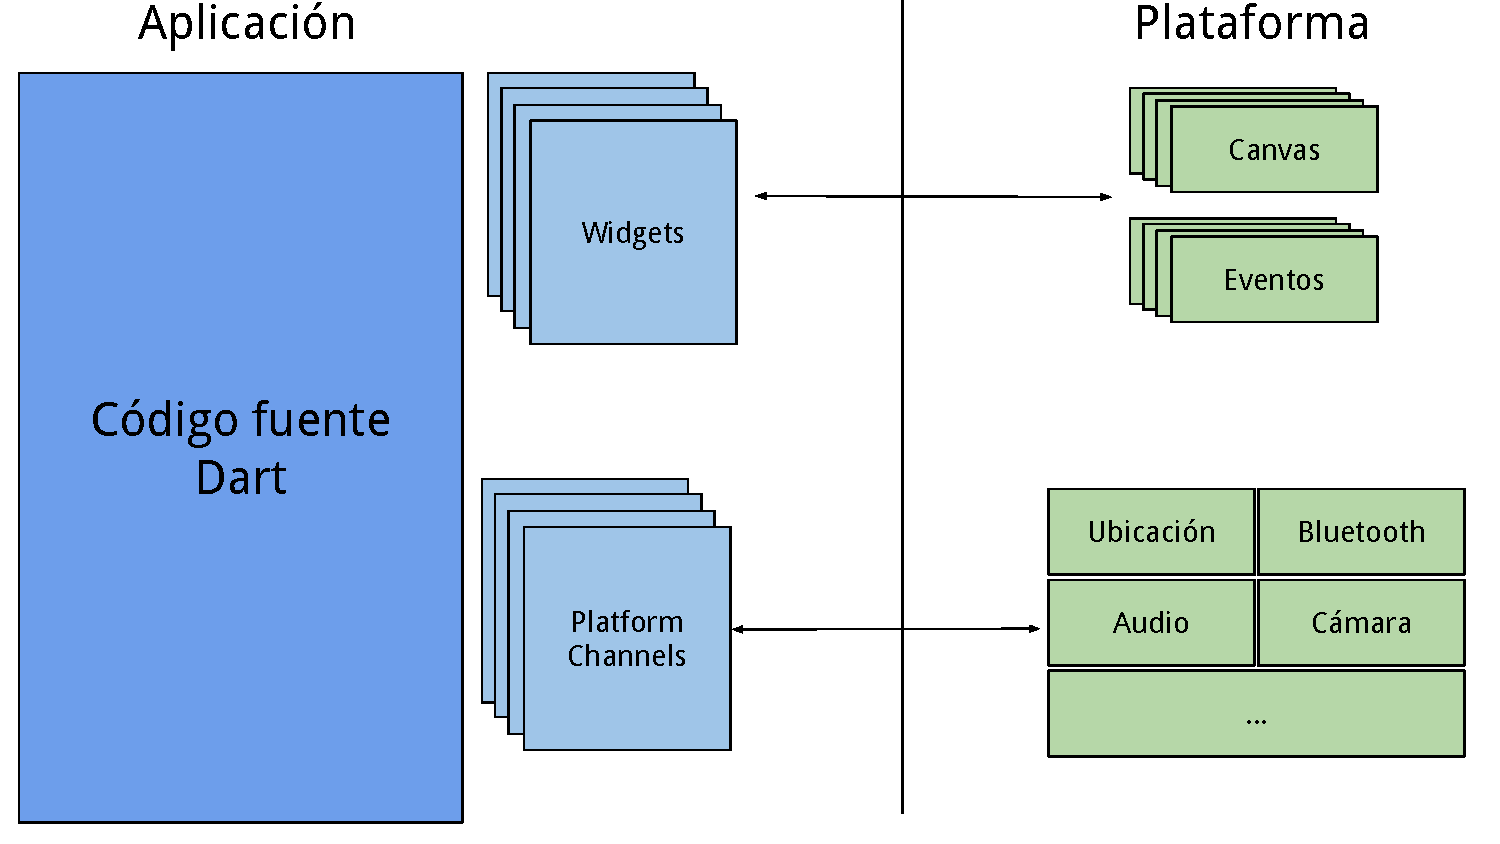
\includegraphics[scale=0.45]{images/flutter1.pdf}
    \caption{Diagrama de renderización de \textit{Flutter}\cite{leler2019s}}
    \label{fig:flutter1}
  \end{figure}

Esta relación \textit{apariencia/rendimiento}, la consigue \textit{Flutter} de forma exitosa
\textit{renderizando} directamente sus componentes, 
\textit{widgets}, en un \textit{canvas}, permitiendo visualizar el mismo componente en las diferentes plataformas.

Del mismo modo, realiza la conversión directa de servicios propios, \textit{Platform Channels}, en librerías nativas que
interactúan con las funcionalidades propias del dispositivo~\cite{leler2019s}, 
tal y como se puede visualizar en la Figura \ref{fig:flutter1}.

Esta en una de las razones principales por las que se ha elegido el uso de este herramienta frente a otros 
\textit{frameworks} de desarrollo móvil como: 

\begin{itemize}
    \item[$\bullet$] \textit{Frameworks de desarrollo móvil basados en Javascript} como: \textit{React Native} y 
    \textit{Vue Native}, que necesitan de una
    capa adicional para realizar la conversión a \textit{componentes nativos}, pudiendo afectar al rendimiento.
    \item[$\bullet$] Los \textit{frameworks embebidos} como
    \textit{Ionic} que emplea un \textit{WebView} para mostrar los componentes, dando la sensación que no estás ejecutando
    una aplicación móvil, sino un sitio web embebido.
 \end{itemize}

 \subsection{Firebase}
 Para todas las funcionalidades relacionadas con servicios \textit{en nube}, vistos en la fase de Análisis,
 se empleará la plataforma de desarrollo backend impulsada y recomendada por \textit{Google}: \textit{Firebase}.

Gracias a que \textit{Firebase} presenta una base de datos del tipo \textit{real-time}, permitirá 
la sincronización de los datos durante la ejecución del
aplicativo~\cite{khawas2018application}. Esta característica resulta ideal, ya que
\textit{Flutter} al tratarse de un \textit{framework "declarativo"} no requiere de eventos para
sincronizar los datos, permitiendo al usuario visualizar los datos, en todo momento, sincronizados en pantalla,
sin necesidad de que el usuario realice un \textit{input de refrescar}.

Resulta muy potente esta propiedad, ya que la han querido adoptar los frameworks de desarrollo móvil nativo principales,
con aproximaciones como: \textit{SwiftUI} para aplicaciones \textit{iOS} y \textit{Jetpack Compose} para soluciones \textit{Android}.

Además, esta, al pertenecer al tipo de las \textit{no relacionales}, presenta ciertos beneficios frente a 
las \textit{relacionales},
a tener en cuenta en la definición de los modelos, tales como flexibilidad, seguridad y rendimiento.

La funcionalidades \textit{in-cloud} del \textit{back-end} de la aplicación final 
quedarán cubiertas por los apartados mostrados en la Tabla \ref{fig:tableFirebase}

\begin{table}[H]
    \centering
    \caption{Funcionalidades \textit{en nube} cubiertas por \textit{Firebase}}
      \begin{tabular}{ | c | c |}
        \hline
        \thead{Funcionalidad} & \thead{Tecnología} \\
        \hline
        \makecell{Autentificación} &  \makecell{\textbf{Firebase Authentication}, permite al usuario el acceso a las funciones de \\ la plataforma
        mediante inicio sesión tradicional \\ (cuenta de correo y contraseña)  o por RRSS.} \\
        \hline
        \makecell{Base de datos} &   \makecell{\textbf{Firebase Firestore}, permite al usuario interactuar mediante \\ funciones CRUD 
        la base de datos del sistema.} \\
        \hline
        \makecell{Analíticas} &  \makecell{\textbf{Firebase Analytics}, monitoriza la experiencia de usuario y extrae\\ estadísticas de cara 
        al lanzamiento de futuras versiones tales como:\\ porcentaje de usuarios libre de errores y número de usuarios activos.} \\
        \hline
      \end{tabular}
      \label{fig:tableFirebase}
  \end{table}

El diagrama de flujo del aplicativo con los servicios que ofrece la plataforma \textit{Firebase} puede verse
representado por el diagrama de la Figura\ref{fig:backdiagram1}

\begin{figure}[H]
  \centering
  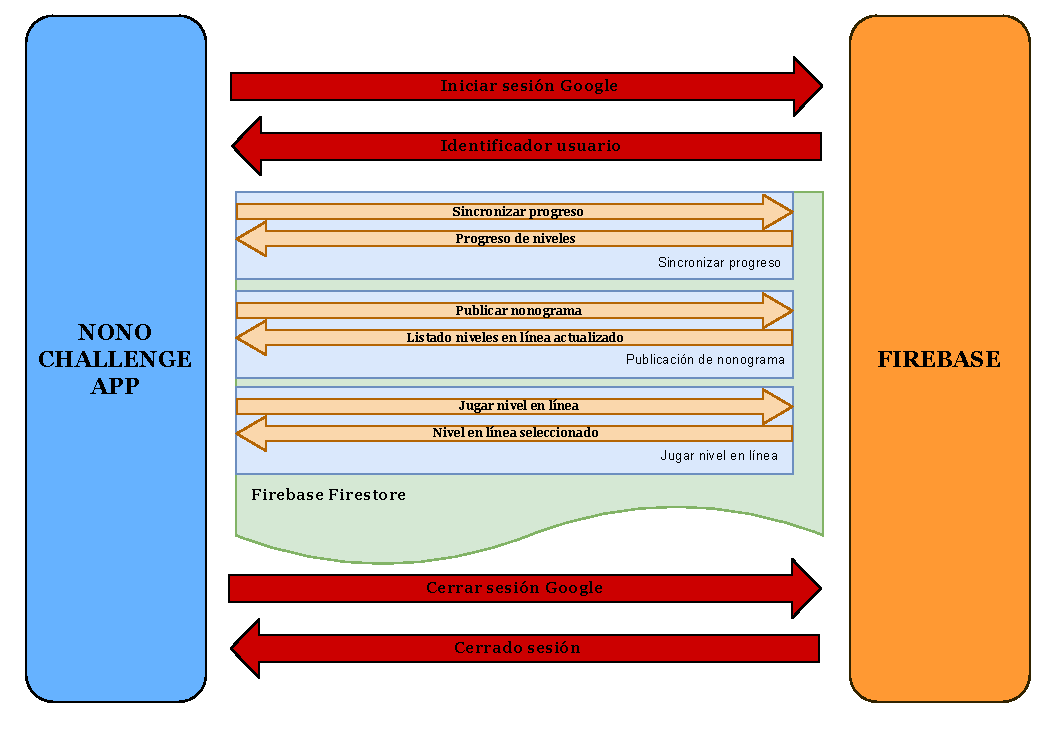
\includegraphics[scale=0.8]{images/back_diagram.pdf}
  \caption{Diagrama de flujo con \textit{Firebase}}
  \label{fig:backdiagram1}
\end{figure}

La gestión del progreso y publicación/resolución de niveles en línea se realizará mediante la función de \textit{Cloud Firestore},
para ello todas las transacciones se realizarán a través del identificador único de usuario.

\begin{figure}[H]
  \centering
  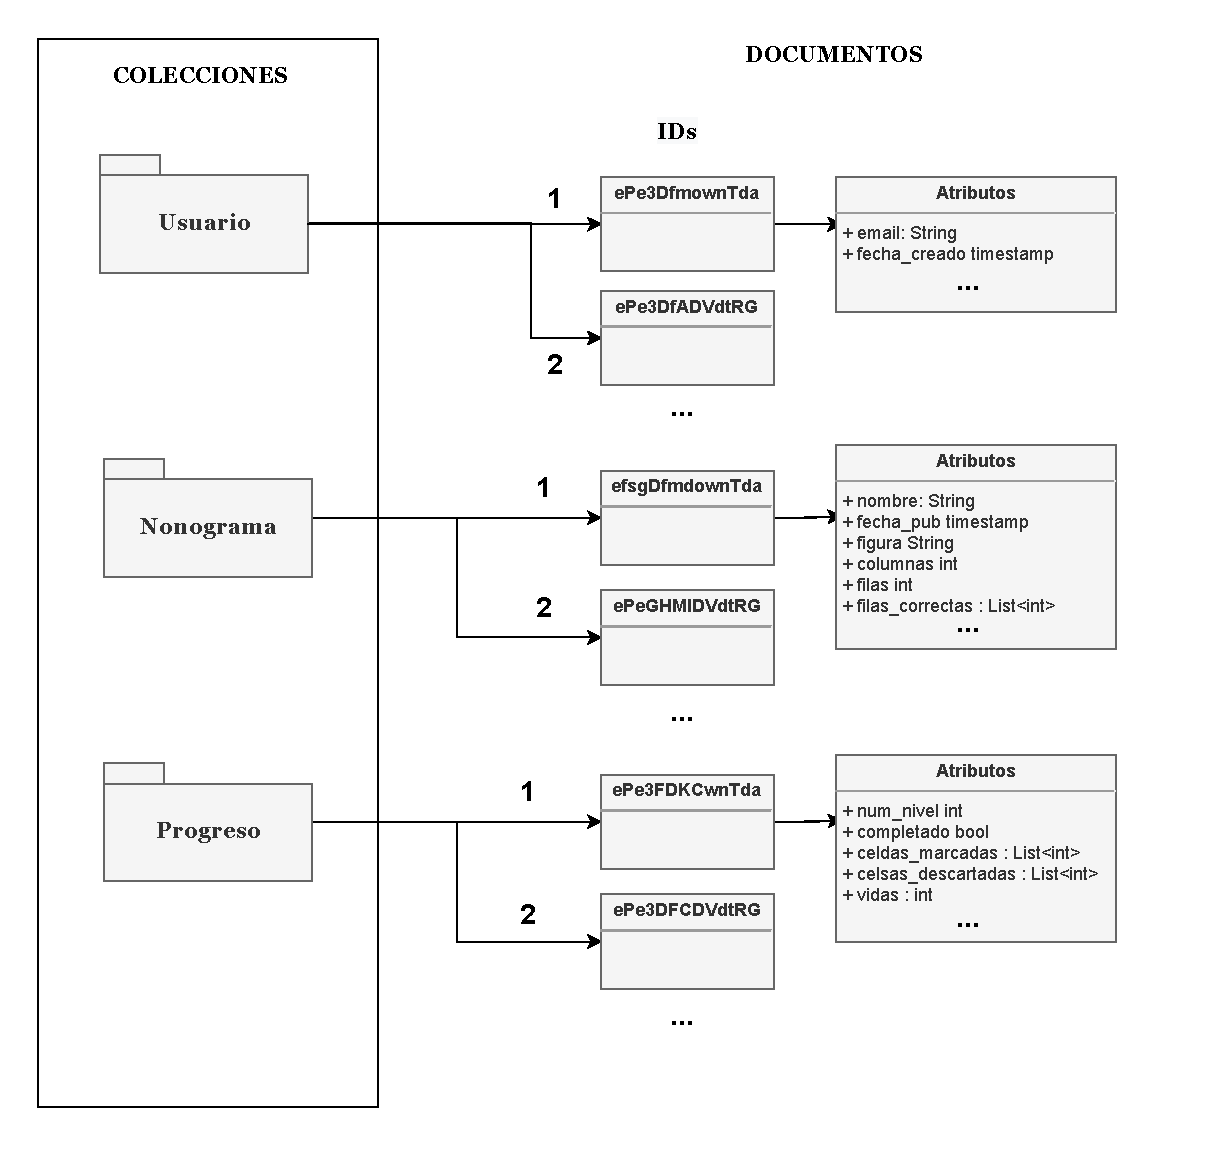
\includegraphics[scale=0.55]{images/firestore.pdf}
  \caption{Diagrama de estructura de datos de \textit{Firestore}}
  \label{fig:firestore1}
\end{figure}

En cuanto a la estructuración de los datos, al tratarse de una base de datos no relacional,
de tipo \textit{NoSql}, se tratarán los datos en forma de \textit{documentos}, cada uno con una clave identificativa única y una
serie de atributos. Estos documentos se almacerán según su tipo en contenedores llamados \textit{colecciones}:
\textit{usuarios, nonogramas y progresos}, en el caso de este aplicativo.

Este modelo de datos, a diferencia de los relacionales puede ser totalmente flexible y definido por el aplicativo, no obstante,
para asegurar una mayor consistencia se ha definido desde el portal web de \textit{Firestore}, Figura \ref{fig:firestore1}.

  \subsection{Visual Studio Code}
Como \textit{IDE} de desarrollo se empleará la herramienta \textit{Visual Studio Code}, desarrollado por
\textit{Microsoft}, frente a otros entornos como: \textit{XCode} y \textit{Android Studio}, ya que este dispone
de una gran cantidad de \textit{extensiones o plugins} que facilitan notablemente el proceso de \textit{codificación},
además de estar mejor optimizado para labores de \textit{compilación y depuración.}

\subsection{GitHub}
Se empleará \textit{GitHub} para el \textit{control de versiones}, siguiendo la metodología propias de 
\textit{GitFlow}, en el que tendremos, como se puede visualizar en la Figura~\ref{fig:gitflow1}:
i) una rama \textit{master} para versiones finales del aplicativo,
ii) una rama \textit{develop} en la que aunar las funcionalidades desarrolladas y iii) las ramas
\textit{feature} que se crearán por cada funcionalidad a desarrollar, dividida por todas las capas propuestas
por la filosofía \textit{Clean Architectute}, junto a sus \textit{suites de tests}.

\begin{figure}[H]
    \centering
    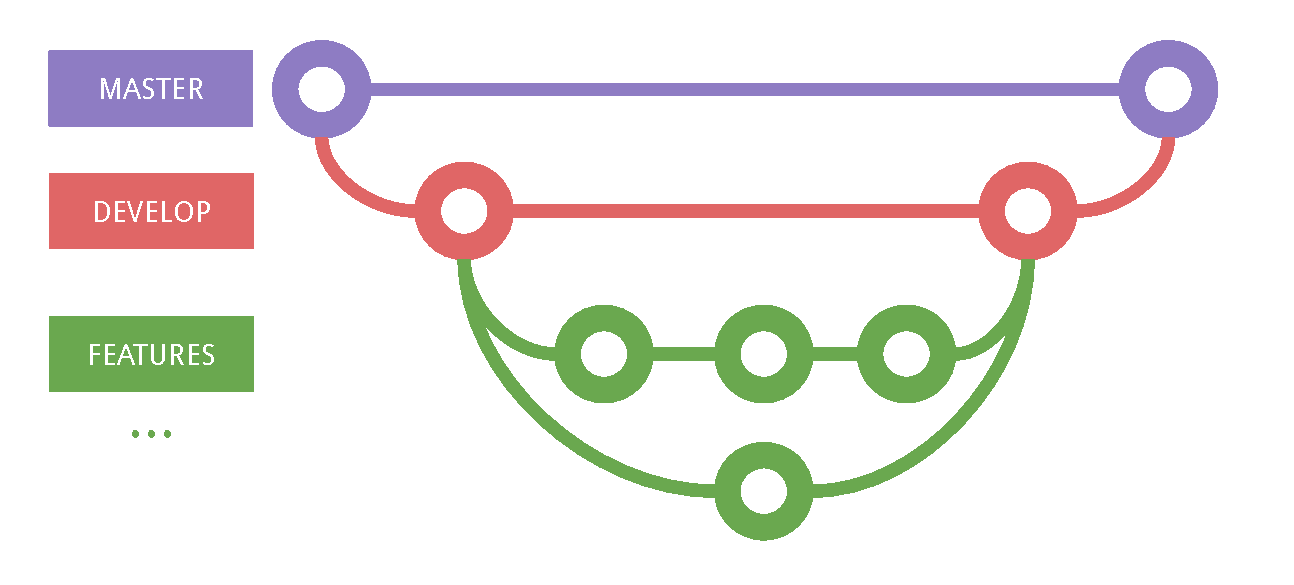
\includegraphics[scale=0.6]{images/gitflow1.pdf}
    \caption{Diagrama del funcionamiento de \textit{GitFlow}}
    \label{fig:gitflow1}
  \end{figure}

Además, nos nutriremos de las buenas prácticas, \textit{librerías} y \textit{repositorios} disponibles en la plataforma,
aprovechando la subida exponencial de la comunidad \textit{Flutter} en este último año, posicionándose
dentro de las tecnologías con más \textit{stars} en el \textit{sitio web}~\cite{gittracker}.

\section{Arquitectura del Sistema}
Una vez definidas las tecnologías que se van a utilizar para el desarrollo de la solución, es importante definir una 
arquitectura que encaje dentro del abanico de requisitos que se desean incluir, además de las funcionalidades que
aportan las tecnologías estudiadas.

Se requiere de una arquitectura de \textit{software} que no tenga tanta complejidad, ya que no se trata de un
proceso industrial y el desarrollo va a ser realizado por una persona, además de estar bien establecida, ya que
no se quiere entorpecer la escalabilidad del sistema, facilitando, de esta forma, las fases de testeo y mantenimiento.

Para un desarrollo con \textit{Flutter} como \textit{framework} de desarrollo \textit{front-end} y \textit{Firebase}
como infraestructura de servicios \textit{back-end}, se empleará, \textit{la arquitectura por capas}, o 
\textit{Layered Architecture} 
una de las más arquitecturas más conocidas y elegidas en entornos de desarrollo móvil~\cite{7053865}.

\subsection{Arquitectura por capas}
El objetivo de esta arquitectura es la de abstraer lo máximo posible los diferentes bloques o componentes que van a
conformar el sistema. 

Empleando la siguiente arquitectura se pretenderá obtener, a corto y largo plazo,  los siguientes beneficios:

\begin{itemize}
  \item[$\bullet$] Componentes que desempeñan una única funcionalidad bien definida.
  \item[$\bullet$] Mayor escalabilidad, favoreciendo la inclusión de nuevas funcionalidades.
  \item[$\bullet$] Facilidad en la identificación de posibles \textit{bugs} o errores relativos a la
  ejecución del aplicativo.
  \item[$\bullet$] Permite la inclusión de \textit{patrones de diseño} en el sistema.
  \item[$\bullet$] Código más legible y fácil de entender.
\end{itemize}

Mediante esta arquitectura es posible dividir el sistema mediante N bloques, para el aplicativo final se ha optado por una
arquitectura dividida en cuatro capas, como se puede visualizar en la Figura~\ref{fig:architecture1}.

\begin{figure}[H]
  \centering
  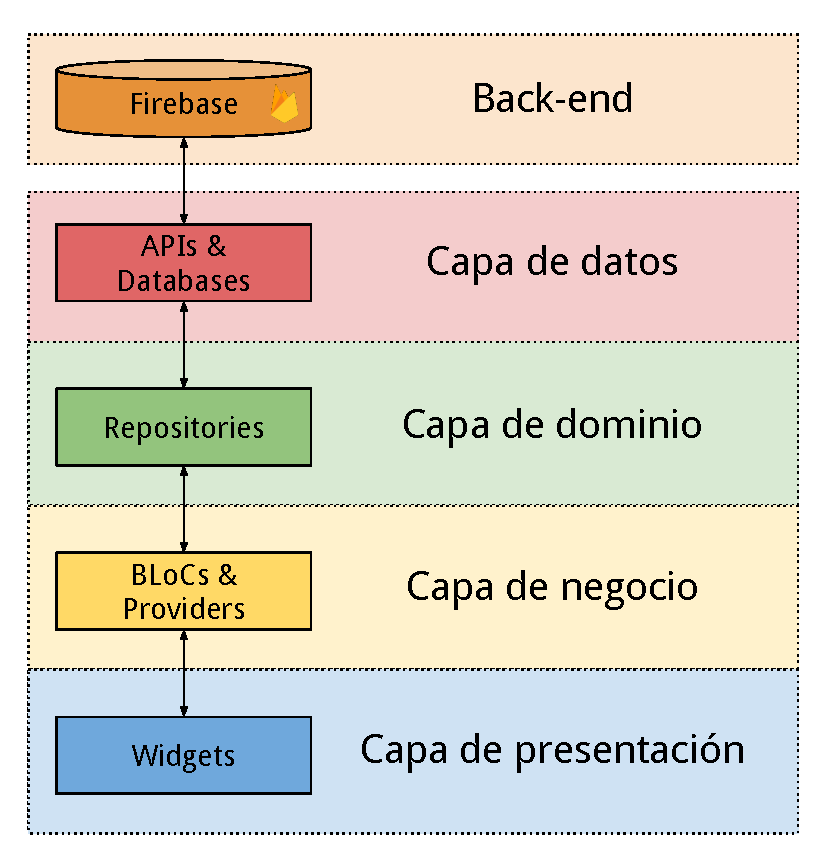
\includegraphics[scale=0.7]{images/architecture.pdf}
  \caption{Diagrama de \textit{Arquitectura basada en cuatro capas}}
  \label{fig:architecture1}
\end{figure}

A continuación, se comentará la funcionalidad de cada una de las capas, en la Tabla~\ref{fig:tablelayers}:

\begin{table}[H]
  \centering
  \caption{Función de las capas de la arquitectura del sistema}
    \begin{tabular}{ | c | c |}
      \hline
      \thead{Capa} & \thead{Funcionalidad} \\
      \hline
      \makecell{Capa de \\ presentación} &  \makecell{Mediante \textit{widgets} se presentarán todas las vistas
      y componentes\\ que contiene el aplicativo.} \\
      \hline
      \makecell{Capa de \\ lógica} &   \makecell{A partir de \textit{manejadores de estados} se controlarán todos los \\ cambios de
      estado presentes en la capa de \textit{presentación}.} \\
      \hline
      \makecell{Capa de \\ dominio} &  \makecell{Las interfaces \textit{repositorio} servirán de esqueleto \\ para las clases relacionadas con
      la capa de \textit{datos}.} \\
      \hline
      \makecell{Capa de \\ datos} &  \makecell{Implementando las interfaces de la capa de \textit{dominio} se
      obtendrán los \\ datos de fuentes externas como nuestro \textit{back-end} de \textit{Firebase}} \\
      \hline
    \end{tabular}
    \label{fig:tablelayers}
\end{table}

Adicionalmente, justo a este modelo de capas se adoptará
la arquitectura \textit{Clean Arquitecture} y la metodología de desarrollo quiado
por pruebas \textit{TDD}, práctica cada vez más vista en proyectos extensos y de gran escalabilidad ~\cite{9071367}.
La combinación de estas dos praxis, permitirán modularizar al máximo las funcionalidades del sistema, haciéndolos más
reutilizables y fáciles de monitorizar en las tareas de identificación de errores y rendimiento.

\subsection{Manejador de estados}

Es cierto que \textit{Flutter}, permite \textit{manejar} todos los diferentes \textit{estados} que van surgiendo
en el aplicativo, como por ejemplo: \textit{refresar de forma dinámica una lista de objetos}; directamente
en la \textit{capa de presentación}, mediante la función \textit{setState()}\cite{flutterState}.

Sin embargo, para nuestra aplicación u otras soluciones de gran envergadura esta tarea puede resultar muy compleja,
además de ser totalmente opuesta a la modulabilidad y reusabilidad que ofrece la arquitectura \textit{Clean Architecture}.
Por ello, se hacen necsearios patrones de diseño que actúen como
\textit{manejadores de estados}, que esté presente en la capa de \textit{lógica} y que se encarguen de:

\begin{itemize}
  \item[$\bullet$] Controlar todos los eventos presentes en el aplicativo 
  para transformarlos en estados y transmitirlos a la capa de \textit{presentación}.
  \item[$\bullet$] Obtener los datos sincronizados transmitidos por la capa de \textit{datos}.
\end{itemize}

Dentro del gran abanico de librerías e implementaciones que ofrece \textit{Flutter} se ha optado por, como se puede 
visualizar en la Figura~\ref{fig:architecture1}, la combinación de los siguientes patrones:

\begin{itemize}
  \item[$\bullet$] \textbf{Patrón BLoC}: empleado para centralizar los cambios de estado, recibiendo \textit{eventos}
   de la capa de \textit{presentación} y transmitir \textit{estados} que cambien de forma dinámica los componentes de
    la misma.
  \item[$\bullet$] \textbf{Provider}: nos permitirá, como su nombre indica, proveer de funcionalidades propias
  de la capa de lógica, como la lógica de los BLoCs a la \textit{capa de presentación}.
\end{itemize}

Esta combinación de patrones se incluirá en el aplicativo mediante el paquete \textit{flutter\_bloc}.
En el capítulo de \textit{Desarrollo de la solución}, se podrá visualizar algunos ejemplos de dicha metodología en
el sistema.


\chapter{Desarrollo de la solución}
\textit{El desarrollo de aplicaciones móviles resulta desafiante por la gran variedad de dispositivos
móviles con diferentes sistemas operativos, características y tamaños \cite{7021823}. Esta tarea
la suplementa Flutter con sus widgets, permitiendo
desarrollar todo tipo de vistas con un diseño adaptativo para la mayoría de dispositivos.
}

\section{Prototipado de pantallas}
El diseño de la totalidad de pantallas se ha realizado siguiendo las pautas y directrices marcadas por
el estándar \textit{Material Design}. Su gran contenido de iconos, estilos y componentes se ha plasmado,
gracias al paquete \textit{material}, directamente en el aplicativo.

Antes del desarrollo completo de cada una de las pantallas del aplicativo, se ha optado por el diseño de
\textit{MockUps}, indicando cada uno de los casos de uso y requisitos funcionales vistos en el Capítulo 
3, indicados por los identificadores del \textit{1 al 21}.

\begin{figure}[H]
    \centering
    \begin{subfigure}[b]{0.38\linewidth}
      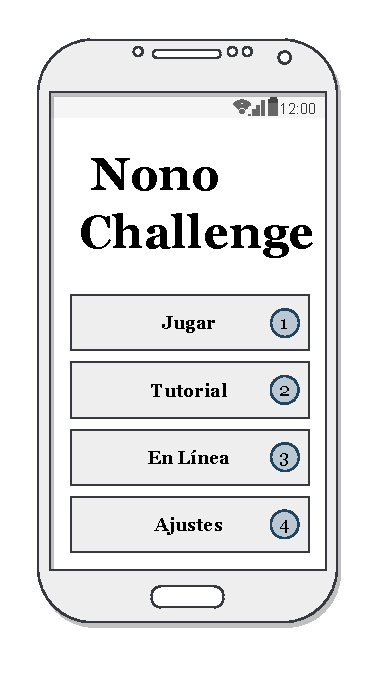
\includegraphics[width=\linewidth]{images/screen1.pdf}
    \end{subfigure}
    \begin{subfigure}[b]{0.38\linewidth}
      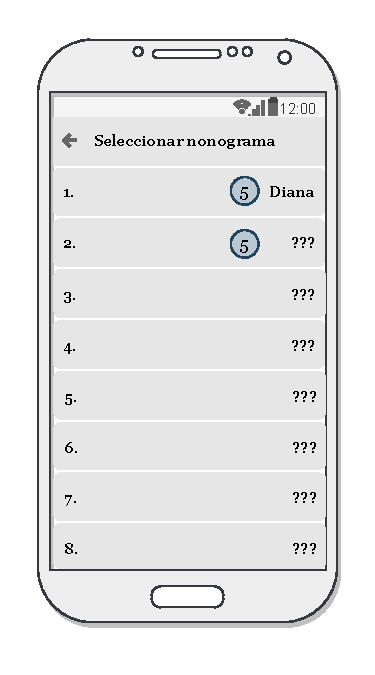
\includegraphics[width=\linewidth]{images/screen2.pdf}
    \end{subfigure}
    \caption{MockUps Pantalla de Inicio y Selector de niveles clásicos}
    \label{fig:design-1}
\end{figure}

La Pantalla de Inicio será la encargada de proveer al usuario el acceso de todos los casos
de uso y requisitos funcionales disponibles.

La pantalla de Selector de niveles clásicos mostrará todos los niveles disponibles predeterminados del sistema,
muchos de ellos extraídos de los libros \textit{Griddlers}, publicados por el noticiero británico 
\textit{Sunday Telegraph}.
A medida los niveles han sido superados se descubrirá el nombre de la figura que representa, Figura \ref{fig:design-1}.

\begin{figure}[H]
    \centering
    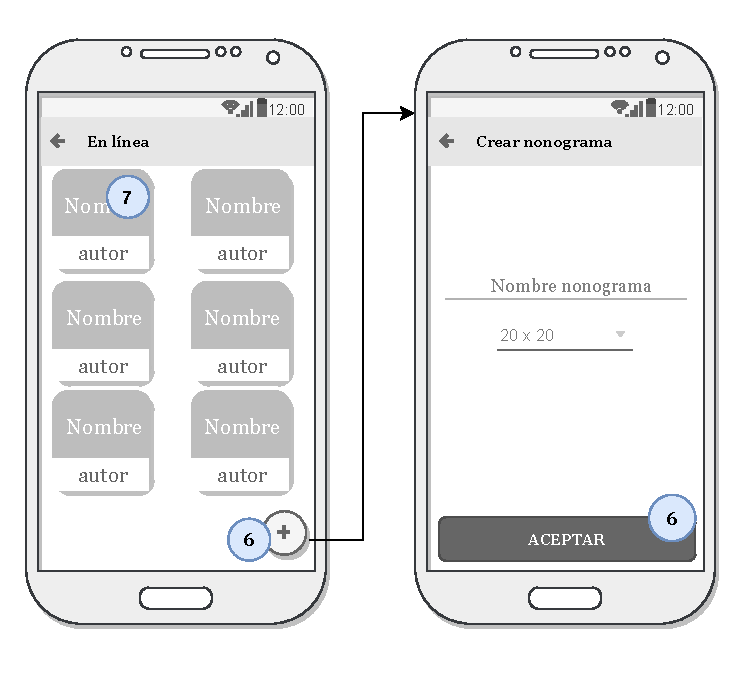
\includegraphics[scale=0.83]{images/screen3.pdf}
    \caption{MockUps Pantalla de niveles online y publicación de nonogramas}
    \label{fig:design-2}
\end{figure}

\begin{figure}[H]
  \centering
  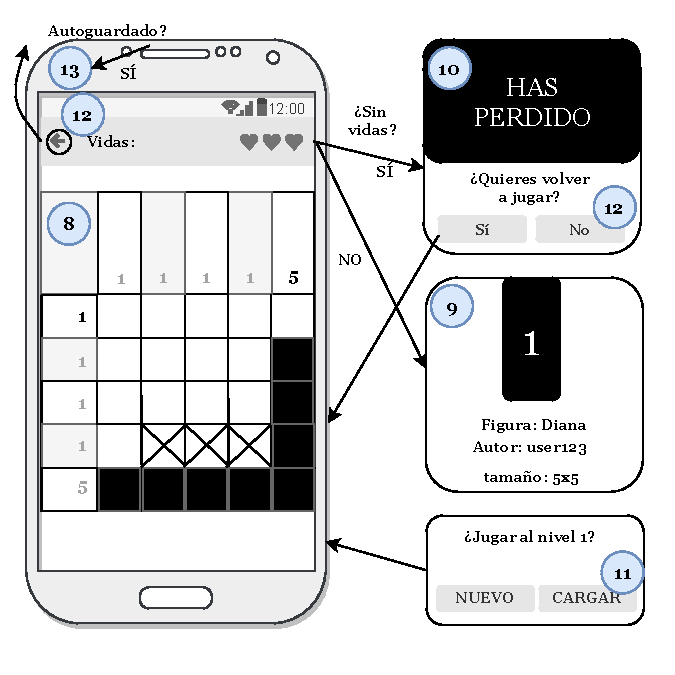
\includegraphics[scale=0.83]{images/screen4.pdf}
  \caption{MockUp Pantalla de resolución de nivel}
  \label{fig:design-3}
\end{figure}

En la Figura \ref{fig:design-3} se puede observar el diagrama de flujo de resolución
de nivel. 
Como se puede apreciar, la apariencia y esencia del rompecabezas es fiel al de los medios tradicionales:

\begin{itemize}
  \item[$\bullet$] Las celdas pintadas representan las celdas que se han seleccionado (con un clic) y
  resultan correctas
  \item[$\bullet$] Aquellas celdas con \textit{equis} son las marcadas  por el
  usuario (con doble clic sobre ella), asegurando que no son correctas.
  \item[$\bullet$] Los bloques de los extremos contienen el número
  de celdas correctas de esa fila o columna, los cuales se van difuminado a medida que se van
  resolviendo por el usuario.
\end{itemize}

El jugador puede abandonar el nivel en cualquier momento, guardando su progreso si la opción de autoguardado
está activada. En el instante de resolverlo satisfactoriamente (con al menos una vida) se mostrarán
las características del mismo, y en el caso contrario, la opción de volver a intentarlo.

\begin{figure}[H]
  \centering
  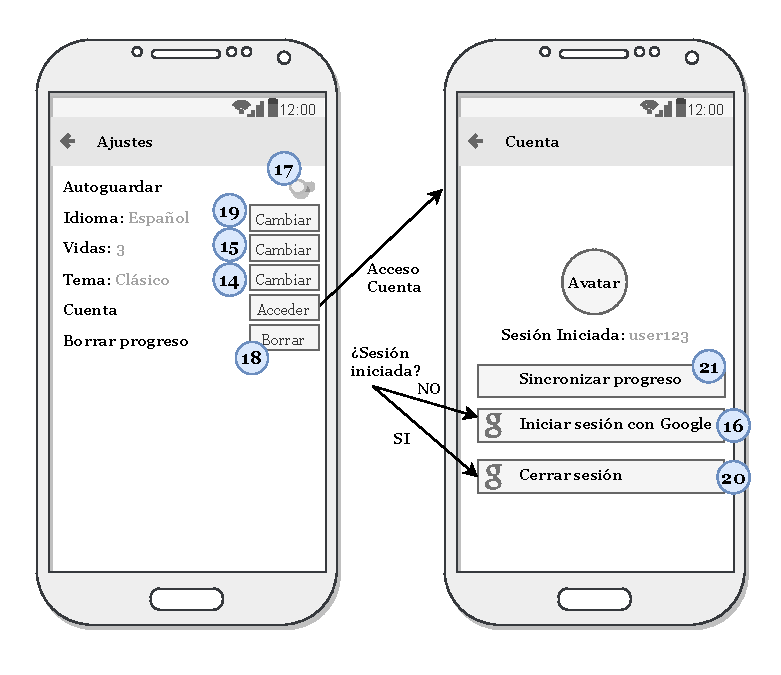
\includegraphics[scale=0.83]{images/screen5.pdf}
  \caption{MockUp Pantalla de ajustes y cuenta}
  \label{fig:design-4}
\end{figure}

En la pantalla se pueden configurar propiedades relativas a: 

\begin{itemize}
  \item[$\bullet$] La experiencia de juego como: la posibilidad de autoguardado y
  el número de vidas.
  \item[$\bullet$] El idioma de la totalidad del sistema, por ahora para este \textit{MVP}, entre español e inglés.
  \item[$\bullet$] La combinación de colores que componen el tema del aplicativo.
\end{itemize}

El usuario puede borrar el progreso de todos sus niveles jugados mediante la opción de borrar
progreso, además de sincronizarlo con el \textit{servicio en nube} desde el apartado cuenta, 
iniciando sesión previamente (Figura \ref{fig:design-4})

\section{Estructura del proyecto}
Es importante que en un desarrollo de software se establezca una estructura propia de la arquitectura elegida,
para mantener una modularidad y escalabilidad a nivel de sistema.
Para ello, siguiendo las directrices del modelo \textit{Clean Architecture}, se ha definido el siguiente
árbol de directorios:

\definecolor{folderbg}{RGB}{230,230,230}
\definecolor{folderborder}{RGB}{110,144,169}

\def\Size{4pt}
\tikzset{
  folder/.pic={
    \filldraw[draw=folderborder,top color=folderbg!50,bottom color=folderbg]
      (-1.05*\Size,0.2\Size+5pt) rectangle ++(.75*\Size,-0.2\Size-5pt);  
    \filldraw[draw=folderborder,top color=folderbg!50,bottom color=folderbg]
      (-1.15*\Size,-\Size) rectangle (1.15*\Size,\Size);
  }
}
\begin{figure}[H]
\begin{center}
\begin{forest}
  for tree={
    font=\scriptsize\ttfamily,
    grow'=0,
    child anchor=west,
    parent anchor=south,
    anchor=west,
    calign=first,
    inner xsep=7pt,
    edge path={
      \noexpand\path [draw, \forestoption{edge}]
      (!u.south west) +(7.5pt,0) |- (.child anchor) pic {folder} \forestoption{edge label};
    },
    before typesetting nodes={
      if n=1
        {insert before={[,phantom]}}
        {}
    },
    fit=band,
    before computing xy={l=15pt},
  }  
[nonochallenge
  [assets ----imágenes{,} iconos{,} y fuentes.
  ]
  [lib ----código fuente dart.
    [api ----funciones y llamadas Firebase.
    ]
    [common ----archivos globales del sistema.
      [theme  ----temas del aplicativo.
      ]
      [utils  ----funciones de utilidad.
      ]
      [widgets  ----widgets comunes del sistema.
      ]
    ]
    [core ----clases genéricas de funcionalidad.
      [error ----clases error y excepciones.
      ]
      [platform ----detección de conexiones ej:internet.
      ]
      [usecase ----definición casos de uso.
      ]
    ]
    [di ----inyector de dependencias.
    ]
    [features ----funcionalidades del sistema.
      [feature1 ----funcionalidad.
        [data ----capa de datos.
          [datasources ---- comunicación con Firebase y base de datos local.
          ]
          [models ----implementación de las entities con serialización y funciones.
          ]
          [repositories\_impl ----implementación de los repositorios de dominio.
          ]
        ]
        [domain ----capa de dominio.
          [entities ----modelos de datos.
          ]
          [repositories ----definición genérica de repositorio.
          ]
          [usecases ----definición de los casos de uso de la funcionalidad.
          ]  
        ]
        [presentation ----capa de presentación y lógica.
          [bloc ----manejador de estados y capa de lógica.
          ]
          [pages ----pantallas de la característica.
          ]
          [widgets ----componentes que componen las pantallas.
          ]
        ]
      ]
      [... ----más funcionalidades.
      ]
    ]
    [i10n ----archivos de traducción.
    ]
  ]
  [tests ----tests del sistema
    [feature1 ----suites de test de funcionalidad: unitarios{,} lógica y widgets.
    ]
    [...
    ]
  ]
]
\end{forest}
\label{fig:tree-1}
\caption{Estructura de directorios de \textit{nonogramchallenge}}
\end{center}
\end{figure}

\section{Codificación del aplicativo}
El proceso de codificación se ha realizado posteriormente a la creación de una \textit{suite de tests} de funcionalidades, siguiendo las pautas y
reglas establecidas por la metodología TDD, proceso documentado en el sexto capítulo.

En el siguiente apartado se explicará el \textit{modus operandi} de la codificación de funcionalidades, acompañado de ejemplos definidos 
en el \autoref{cap:anexo2}, comenzando por la capa de presentación.

\subsection{Desarrollo de la capa de presentación}
La creación de cada una de las pantallas y sus componentes se ha realizado, como no podría ser de otra forma, a partir de un \textit{árbol de widgets}. 
Para el desarrollo de pantallas se ha optado por usar widgets inmutables, llamados, \textit{stateless}, en contraposición a los de tipo \textit{stateful},
con estado mutable. \cite{10.1007/978-981-15-1465-4_56} 

Esta práctica permitirá que la \textit{capa de presentación} contenga la mínima lógica posible, pudiendo en un futuro reutilizarla
en otras funcionalidades del sistema o incluso en otras soluciones.

\begin{figure}[H]
  \centering
  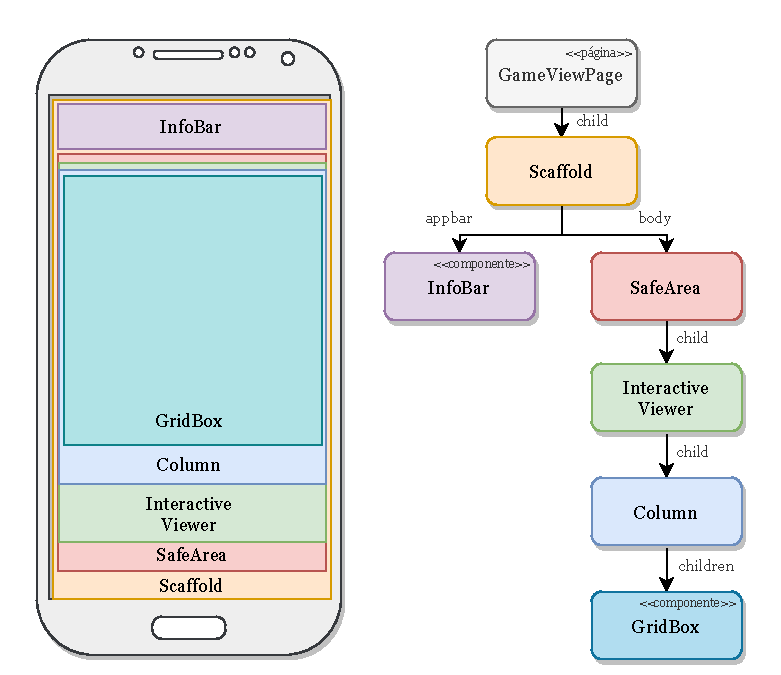
\includegraphics[scale=0.83]{images/treewidgets.pdf}
  \caption{Árbol de widgets Pantalla de Resolución de nivel}
  \label{fig:tree-widgets-1}
\end{figure}

En la Figura \ref{fig:tree-widgets-1} y \autoref{cap:anexo1-1} se puede visualizar el \textit{árbol de widgets} de la pantalla de resolución de nivel, los cuales
se ``construyen'' mediante el método \textit{build()}.

Esta vista contiene algunos widgets de interés que se han usado para mejorar la experiencia de usuario como:
\begin{itemize}
  \item[$\bullet$] \textit{SafeArea}: contenedor que acopla la pantalla en el caso que el dispositivo contenga elementos físicos como \textit{notch}, 
  statusbar, marcos de pantalla redondeados...
  \item[$\bullet$] \textit{InteractiveViewer}: permite al usuario realizar gestos como acercar, alejar y mover el rompecabezas 
  para casos en los que el \textit{nonograma} es de grandes dimensiones. 
\end{itemize}

\subsection{Desarrollo de la capa de lógica}
Para implementar la capa de lógica, se usará el paquete \textit{flutter\_bloc}, para ello se definirán todos los 
posibles estados y eventos presentes en dicha funcionalidad y una clase \textit{BLoC} que se encargue de 
``manejar'' el flujo de cambios de estado.

A continuación, se mostrará un diagrama de flujo de estados de la funcionalidad \textit{lista de nonogramas en línea}.

\begin{figure}[H]
  \centering
  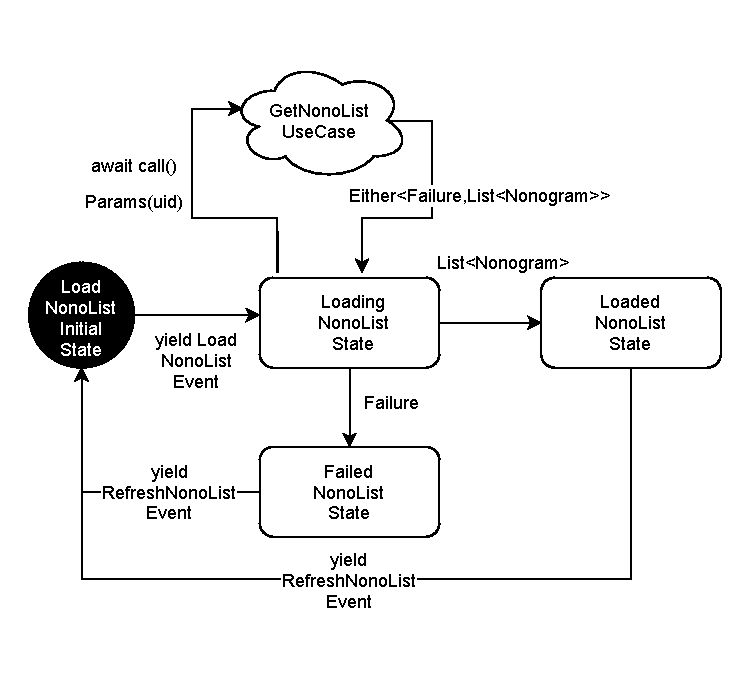
\includegraphics[scale=0.83]{images/statesNonoList.pdf}
  \caption{Diagrama de estado de la funcionalidad Lista de nonogramas en línea}
  \label{fig:nonolist-states}
\end{figure}

Cuando el usuario accede a la sección de nonogramas en línea se manejará, por defecto, el estado
inicial \textit{LoadNonoListInitialState}, que a su vez, enviará el evento \textit{LoadingNonoListEvent}.

En cuanto se envíe tal evento, se tramitará el estado \textit{LoadingNonoListState}, mostrando
un widget de carga.

Durante este estado de ``carga'' pedirá al caso de uso \textit{GetNonoListUseCase} la lista de \textit{nonogramas}
disponible en \textit{Firebase}. Tras esta llamada del caso de uso, nos puede devolver los siguientes
tipos de objeto:

\begin{itemize}
  \item[$\bullet$] La totalidad de \textit{nonogramas} publicados por la comunidad disponible en \textit{Firebase}.
  \item[$\bullet$] Un objeto de tipo \textit{Failure}, indicando que no se ha podido tramitar la operación 
  debido a por ejemplo un error de conexión o de base de datos.
\end{itemize}

En el caso de devolver la lista de \textit{nonogramas} actualizado con éxito, se manejará el estado
\textit{LoadedNonoListState}, mostrando la lista de \textit{rompecabezas} al usuario y en su defecto el estado 
de \textit{FailedNonoListState}, cargando una vista de error. 

El código correspondiente se puede encontrar en
\autoref{cap:anexo1-2}.

\break

\subsection{Desarrollo de la capa de dominio}
El desarrollo de la \textit{capa de dominio} comienza con la definición de casos de uso a usar por el \textit{BLoC}.
Esta implementación se realiza a partir de la clase genérica \textit{usecase} disponible en el paquete \textit{core}.

Como se ha podido comprobar en la \textit{capa de dominio}, este caso de uso devuelve un objeto
de tipo \textit{Either<Failure,Type>}, indicando que puede devolver el tipo de objeto deseado, \textit{Type}, o en caso contrario,
un objeto de tipo \textit{Failure} debido a un error ocurrido en la llamada del repositorio. Adicionalmente, este caso de uso puede
recibir o no una lista de parámetros a usar por el repositorio, como por ejemplo, el \textit{uid} del usuario.

Este aspecto, puede realizarse gracias al paquete externo \textit{dartz}, dotando a \textit{Dart} de aspectos y 
beneficios propios de los lenguajes funcionales.

Una vez definido el caso de uso se definirán las clases genéricas de \textit{repositorios} y \textit{entities} a usar en la
\textit{capa de datos}.

Siguiendo la funcionalidad de \textit{Lista de nonogramas en línea} se puede mostrar la implementación de su \textit{capa 
de dominio} en el \autoref{cap:anexo1-3}.

\subsection{Desarrollo de la capa de datos}
El último paso consiste en desarrollar la \textit{capa de datos} de la funcionalidad, comenzará con la definición de los
\textit{modelos} y la \textit{implementación de los repositorios} a partir de las clases genéricas de \textit{entities} y
\textit{repositories} respectivamente, definidas previamente en la \textit{capa de dominio}.

La implementación de estos \textit{repositorios} emplearán clases de tipo \textit{datasource} que establecerán una conexión
con fuentes de datos externas propias del aplicativo como: i) la base de datos local de la solución y ii) el 
servicio \textit{FireStore} propio de \textit{Firebase}.

Esta \textit{implementación del repositorio} se encargará de
devolver un objeto \textit{Left} o \textit{Right} propio del paquete \textit{dartz}, dependiendo del comportamiento de 
los \textit{datasources} empleados: 

En la funcionalidad citada como ejemplo dichos ejemplos contendrán los siguientes tipos de objeto, tal y como se puede visualizar
en \autoref{cap:anexo1-4}:
\begin{itemize}
  \item[$\bullet$] El objeto \textit{Right} contendrá la lista de nonogramas actualizado obtenido por la llamada a \textit{Firebase} realizada por el 
  \textit{datasource}
  \item[$\bullet$] El objeto \textit{Left} contendrá un \textit{Failure} indicando que no se ha podido tramitar la operación 
  debido a por ejemplo un error de conexión o de base de datos.
\end{itemize}

\subsection{Inyección de dependencias}
Por último, con el fin de ``localizar'' cada una de las capas mencionadas y hacerlas accesibles en cada punto del aplicativo,
se empleará el uso de un \textit{Inyector de dependencias}. 

Esta práctica es altamente recomendable, sobre todo, en soluciones de una
extensión importante. Para ello, se definirá en el directorio \textit{di} del sistema raíz \textit{lib} la clase
\textit{injection\_container.dart}, tal y como se puede visualizar en \autoref{cap:anexo1-5}.

La definición de esta clase se realizará mediante la librería externa \textit{Get\_It}, uno de los \textit{localizadores de servicios}
más popular. En el se crearán \textit{factories} para "inyectar" los \textit{BLoCs} y \textit{singletons} para el resto de
servicios (\textit{repositories},\textit{use cases}, \textit{datasources} y servicios externos como \textit{Firebase} y \textit{Sqflite}).

\APPENDIX
\begin{sidewaysfigure}
\chapter{Diagrama de Gantt del proyecto}
\label{chap:A1}

En el siguiente apéndice se puede observar una evolución de las distintas fases que conforman el proyecto dividas en semanas,
cada una de las fases refleja su tiempo estimado y el tiempo original desde su inicio hasta su finalización.

\definecolor{barblue}{RGB}{153,204,254}
\definecolor{groupblue}{RGB}{51,102,254}
\definecolor{linkred}{RGB}{165,0,33}
\renewcommand\sfdefault{phv}
\renewcommand\mddefault{mc}
\renewcommand\bfdefault{bc}
\setganttlinklabel{s-s}{START-TO-START}
\setganttlinklabel{f-s}{FINISH-TO-START}
\setganttlinklabel{f-f}{FINISH-TO-FINISH}
\begin{ganttchart}[
    canvas/.append style={fill=none, draw=black!5, line width=.75pt},
    hgrid style/.style={draw=black!5, line width=.75pt},
    vgrid={*1{draw=black!5, line width=.75pt}},
    today=7,
    today rule/.style={
      draw=black!64,
      dash pattern=on 3.5pt off 4.5pt,
      line width=1.5pt
    },
    today label font=\small\bfseries,
    title/.style={draw=none, fill=none},
    title label font=\bfseries\footnotesize,
    title label node/.append style={below=7pt},
    include title in canvas=false,
    bar label font=\mdseries\small\color{black!70},
    bar label node/.append style={left=2cm},
    bar/.append style={draw=none, fill=black!63},
    bar incomplete/.append style={fill=barblue},
    bar progress label font=\mdseries\footnotesize\color{black!70},
    group incomplete/.append style={fill=groupblue},
    group left shift=0,
    group right shift=0,
    group height=.5,
    group peaks tip position=0,
    group label node/.append style={left=.6cm},
    group progress label font=\bfseries\small,
    link/.style={-latex, line width=1.5pt, linkred},
    link label font=\scriptsize\bfseries,
    link label node/.append style={below left=-2pt and 0pt}
  ]{1}{13}
  \gantttitle[
    title label node/.append style={below left=7pt and -3pt}
  ]{WEEKS:\quad1}{1}
  \gantttitlelist{2,...,13}{1} \\
  \ganttgroup[progress=57]{WBS 1 Summary Element 1}{1}{10} \\
  \ganttbar[
    progress=75,
    name=WBS1A
  ]{\textbf{WBS 1.1} Activity A}{1}{8} \\
  \ganttbar[
    progress=67,
    name=WBS1B
  ]{\textbf{WBS 1.2} Activity B}{1}{3} \\
  \ganttbar[
    progress=50,
    name=WBS1C
  ]{\textbf{WBS 1.3} Activity C}{4}{10} \\
  \ganttbar[
    progress=0,
    name=WBS1D
  ]{\textbf{WBS 1.4} Activity D}{4}{10} \\[grid]
  \ganttgroup[progress=0]{WBS 2 Summary Element 2}{4}{10} \\
  \ganttbar[progress=0]{\textbf{WBS 2.1} Activity E}{4}{5} \\
  \ganttbar[progress=0]{\textbf{WBS 2.2} Activity F}{6}{8} \\
  \ganttbar[progress=0]{\textbf{WBS 2.3} Activity G}{9}{10}
  {WBS1C}{WBS1D}
\end{ganttchart}
\end{sidewaysfigure}


\chapter{Fragmentos de código}
\label{cap:anexo2}
\textit{La intención de este anexo es la de mostrar algunos ejemplos de código extraídos del 
resultado de la fase de codificación, con el fin de ofrecer un mayor entendimiento de
los pasos realizados para cada una de las funcionalidades desarrolladas.
}

\section{Código de Pantalla de Resolución de Nivel}

\label{cap:anexo1-1}

Este apartado muestra la codificación de la página de la funcionalidad Resolución de nivel, 
(\textit{play\_game\_page.dart}).


\begin{lstlisting}

    import 'package:flutter/material.dart';
    import 'package:flutter_bloc/flutter_bloc.dart';
    
    import '../../../../common/theme/theme.dart';
    import '../widgets/grid_box_view.dart';
    import '../widgets/info_bar_view.dart';
    import '../bloc/play_game_bloc.dart';
    
    class PlayGamePage extends StatelessWidget {
      @override
      Widget build(BuildContext context) {
        var gridBloc = BlocProvider.of<PlayGameBloc>(context);
        var colorSet = ThemeManager.of(context).colorSet;
        return Scaffold(
            appBar: InformationBar(
              mainColor: colorSet.primaryColor,
              sideColor: colorSet.secondaryColor),
            backgroundColor: colorSet.primaryColor,
            body: SafeArea(
                child: InteractiveViewer(
                    maxScale: 3.6,
                    child: Column(
                        mainAxisAlignment: MainAxisAlignment.spaceEvenly,
                        children: [
                          GridBox(
                            width: gridBloc.width,
                            height: gridBloc.height,
                          ),
                        ]))));
      }
    }
    
    \end{lstlisting}

    \section{Código de Capa de Lógica de Niveles En Línea}

    \label{cap:anexo1-2}
    
    El siguiente apartado contiene la codificación de las entidades, repositorios y casos de uso de la 
    funcionalidad \textit{Niveles en Línea}, (\textit{nonolist\_bloc.dart, nonolist\_state.dart y nonolist\_event.dart}).
    
    \begin{lstlisting}
    
    part of 'nonolist_bloc.dart';

    abstract class NonoListState {}
    
    class LoadNonoListInitialState extends NonoListState {}
    
    class LoadedNonoListState extends NonoListState {
      final List<Nonogram> nonograms;
    
      LoadedNonoListState({required this.nonograms});
    }
    
    class FailedNonoListState extends NonoListState {
      final String errorMessage;
    
      FailedNonoListState({required this.errorMessage});
    }
    
    class LoadingNonoListState extends NonoListState {}
    \end{lstlisting}

    \begin{lstlisting}

    part of 'nonolist_bloc.dart';

    abstract class NonoListEvent {}
    
    class LoadNonoListEvent extends NonoListEvent {
      final String uid;
    
      LoadNonoListEvent({required this.uid});
    }
    
    class RefreshNonoListEvent extends NonoListEvent {}
    \end{lstlisting}

    \begin{lstlisting}

    import 'dart:async';
    import 'package:bloc/bloc.dart';
    import 'package:meta/meta.dart';
    
    import '../../../../core/usecase/usecase.dart';
    import '../../domain/entities/nonogram.dart';
    import '../../domain/usecases/get_online_nonograms_use_case.dart';
    part 'nonolist_event.dart';
    part 'nonolist_state.dart';
    
    class NonoListBloc extends Bloc<NonoListEvent, NonoListState> {
      NonoListBloc({required this.getNonoListUseCase}) : super(LoadNonoListEvent());
    
      final GetNonoListUseCase getNonoListUseCase;
    
      @override
      Stream<NonoListState> mapEventToState(
        NonoListEvent event,
      ) async* {

        if (event is LoadNonoListEvent) {
          final data = await getNonoListUseCase.call(event.uid);
            yield data.fold(
              (left) => FailedNonoListState(errorMessage: left),
              (right) => FailedNonoListState(nonograms: right));
        }
        if (event is RefreshNonoListEvent) {
          bloc.add(LoadNonoListEvent(event.uid));
        }
      }
    }
    \end{lstlisting}

    \section{Código de Capa de Dominio de Niveles En Línea}

    \label{cap:anexo1-3}
    
    Este apartado contiene la codificación de las entidades, repositorios y casos de uso de la 
    funcionalidad \textit{Niveles en Línea}, (\textit{get\_nonolist\_use\_case.dart}, \textit{nonogram.dart} y \textit{nonolist\_repository.dart}).
    
    \begin{lstlisting}
    
    import 'package:dartz/dartz.dart';

    import '../../../../core/error/failures.dart';
    import '../../../../core/usecase/usecase.dart';
    import '../entities/nonogram.dart';
    import '../repositories/nonolist_repository.dart';

    class GetNonoListUseCase extends UseCase<List<Nonogram>, 
      GetNonoListUseCaseParams> {
      final NonoListRepository repository;

      GetNonoListUseCase({required this.repository});
      @override
      Future<Either<Failure, List<Nonogram>>> call
      (GetNonoListUseCaseParams params) async {
        return await repository.getNonoList();
      }
    }

    class GetNonoListUseCaseParams extends Equatable {
      final String uid;

      GetNonoListUseCaseParams({required this.uid});

      @override
      List<Object?> get props => [uid];
    }

    \end{lstlisting}

    \begin{lstlisting}
    
    import 'package:dartz/dartz.dart';

    import '../../../../core/error/failures.dart';
    import '../entities/nonogram.dart';
    
    abstract class NonoListRepository {
      Future<Either<Failure, List<Nonogram>>> getNonoList();
    }    
    \end{lstlisting}

    \pagebreak

    \begin{lstlisting}

    class Nonogram extends Equatable {
      Nonogram({this.id,
        this.solved,
        this.name,
        this.publishDate,
        this.userId,
        this.figure, 
        this.width, 
        this.height, 
        this.correctTiles});
      int? id;
      bool? solved;
      String? name;
      DateTime? publishDate;
      String? userId;
      String? figure;
      String? width;
      String? height;
      List<int>? correctTiles;

      @override
      List<Object?> get props => [id, solved, name, publishDate, userId,
      figure, width, height, correctTiles];
    }
    \end{lstlisting}

    \section{Código de Capa de Datos de Niveles En Línea}

    \label{cap:anexo1-4}
    
    Este apartado contiene la codificación de las entidades, repositorios y casos de uso de la 
    funcionalidad \textit{Niveles en Línea}, (\textit{nonolist\_repo\_impl.dart, nonogram\_model.dart}
    \linebreak y \textit{nonolist\_data\_source.dart}).
    
    \begin{lstlisting}
      
    import 'package:dartz/dartz.dart';
    import '../../../../core/error/exceptions.dart';
    import '../../../../core/error/failures.dart';
    import '../../domain/repositories/nonolist_repo_impl.dart';
    import '../model/nonogram_model.dart';
    import '../datasources/nonolist_data_source.dart';
    
    class NonoListRepositoryImpl implements NonoListRepository {
      final NonoListDataSource nonoListDataSource;
      final AuthFirebaseDataSource authDataSource;

      NonoListRepositoryImpl({required this.nonoListDataSource, 
          required this.authDataSource});
      @override
      Future<Either<Failure, List<Nonogram>>> getNonoList() async {
        var authFirebaseInstance;
        try {
          authFirebaseInstance = await authDataSource.getAuthInstace();
        } catch (e) {throw Left(AuthFailure)}
        try {
          final remoteNonoList = 
          await authFirebaseInstance.getRemoteNonolist(
            authFirebaseInstance);
          return Right(remoteNonoList);
        } on ServerException { throw Left(ServerFailure);}}}
    \end{lstlisting}

    \begin{lstlisting}

    class NonogramModel extends Nonogram {
      Nonogram({this.id,
        this.solved,
        this.name,
        this.userId,
        this.publishDate,
        this.figure, 
        this.width, 
        this.height, 
        this.correctTiles}):super(
          id: id,
          solved: solved,
          publishDate: publishDate,
          userId: userId,
          figure: figure,
          width: width,
          height: height,
          correctTiles: correctTiles
        )}
    DocumentReference get ref =>
      FirebaseFirestore.instance.collection('nonograms').doc(id);
      
    static Nonogram fromDoc(DocumentSnapshot data) =>
      Nonogram.createFromData(data.data()!, data.id);

    static Future<QuerySnapshot> getNonoListSorted() {
      return FirebaseFirestore.instance
          .collection('nonograms')
          .orderBy('publish_date')
          .get(dataSource);}
    \end{lstlisting}

    \begin{lstlisting}

    import 'dart:convert';
    
    import '../../../../api/endpoints.dart';
    import '../../../../api/api_configuration.dart';
    import '../../../../core/error/exceptions.dart';
    import '../models/nonogram_model.dart';
    
    abstract class NonoListDataSource {
      Future<NonogramModel> getRemoteNonolist(FirebaseFirestore instance);
    }

    class NonoListDataSourceImpl implements NonoListDataSource {
      @override
      Future<bool> getRemoteNonolist() async {
        final nonolist = 
        await instance
          .collection(NonoCollections.nonograms) //<- "nonograms"
          .get()
        if(nonolist != null) {
          return nonolist;
        } else {
          throw ServerException();
        }
      }
    }
  \end{lstlisting}

  \section{Código Inyector de dependencias}

  \label{cap:anexo1-5}
    
  Este último apartado refleja el \textit{inyector de dependencias} del proyecto,
  mediante la librería externa \textit{get\_it}, donde se ``localizan'' todas
  las capas  (\textit{injection\_container.dart}).

\begin{lstlisting}

  final sl = GetIt.instance;

  Future<void> init() async {
    final sharedPreferences = await SharedPreferences.getInstance();
    final auth = await FirebaseAuth.instance;
    final fireStore = await FirebaseFirestore.instance;
  
    sl
      // External
      ..registerLazySingleton(() => sharedPreferences)
      ..registerLazySingleton(() => auth)
      ..registerLazySingleton(() => fireStore)
  
      // BLoC
      ..registerFactory(() => NonoListBloc(getNonoListUseCase: sl()))
  
      // Use cases
      ..registerLazySingleton(() => GetNonoListUseCase(repository: sl()))

      // Repository
      ..registerLazySingleton<NonoListRepository>(() =>
          NonoListRepositoryImpl(
              nonoListDataSource: sl(),
              authDataSource: sl()))
      
      // Data sources
      ..registerLazySingleton<NonoListDataSource>(
          () => NonoListDataSourceImpl())
  }
  
\end{lstlisting}

%% BIBLIOGRAPHY
%https://stackify.com/what-is-sdlc/

%https://www.tutorialspoint.com/sdlc/sdlc_overview.html

%http://www.umsl.edu/~hugheyd/is6840/waterfall.html

%https://www.inf.upv.es/www/etsinf/wp-content/uploads/2019/03/EstucturayContenidodeunTFGUltimaversion6_3_19.pdf

%https://riunet.upv.es/bitstream/handle/10251/151019/Yerle%20-%20Aplicación%20para%20la%20suscripción%20a%20eventos%20deportivos.pdf?sequence=1&isAllowed=y

%https://riunet.upv.es/bitstream/handle/10251/69088/FRESNEDA%20-%20Aplicación%20de%20patrones%20de%20diseño%20para%20la%20resolución%20de%20problemas%20de%20software%20en%20el%20des....pdf?sequence=2&isAllowed=y

% \end{thebibliography}
\bibliographystyle{IEEEtranS}
\bibliography{bibliography.bib}
\cleardoublepage

%% APPENDIX

% \APPENDIX


%% END

\end{document}
